\documentclass[spanish,draft,12pt,headsepline,footsepline,paper=letter]{scrreprt}
\pagestyle{headings}

\usepackage[utf8]{inputenc}
\usepackage[T1]{fontenc}
\def\spanishoptions{es-noquoting,es-nolists,mexico-com}
\usepackage[spanish]{babel}

\usepackage{makeidx}
\makeindex

\usepackage[nonumberlist]{glossaries}
\makeglossaries

\usepackage[final]{graphicx}
\DeclareGraphicsExtensions{.pdf,.png,.jpg}
\graphicspath{{media/}}
\usepackage{rotating}

\usepackage{scrhack}

\usepackage{natbib}
\usepackage{amsmath,amssymb, bm}
\usepackage{esint}
\usepackage{enumerate}
\usepackage{ragged2e}
\usepackage{nameref}

\usepackage{booktabs}
\usepackage{pdfpages}
\usepackage{setspace}
\onehalfspacing
\frenchspacing
\recalctypearea

\usepackage{marginnote}
% \usepackage{hyperref}

\usepackage{ulem}

\pdfsuppresswarningpagegroup=1
\setlength{\parindent}{0.25in}

\let\olditemize\itemize
\renewcommand{\itemize}{
\olditemize
\setlength{\itemsep}{0pt} 
\setlength{\parskip}{0pt}
\setlength{\parsep}{0pt}
\setlength{\topsep}{0pt}
\setlength{\topmargin}{0pt}  
}

\newenvironment{simple}{\setlength{\parindent}{0pt}}{}

\renewenvironment{quotation}{\list{}{\leftmargin=0.25in}\item[]}{\endlist}

\newcommand{\BigO}{\ensuremath{\mathcal{O}}}% big-O notation/symbol

\addto\captionsspanish{
  \renewcommand\bibname{Referencias}
}
% \renewcommand\textbf{\emph}

\newglossaryentry{asignatura} {
	   name = asignatura,
    description = {Materia que se enseña en un curso y que forma parte de un programa de estudios}}
\newglossaryentry{aula} {
	   name = aula,
    description = {Sala de un centro de enseñanza donde acuden alumnos}}
\newglossaryentry{complecion} {
    name        = compleción,
    description = {Calidad o condición de completo:aquella destrucción no se llevaba a efecto con el rigor y la compleción debidos}}
\newglossaryentry{clase} {
           name = clase,
    description = {Conjunto de escolares o estudiantes de un mismo nivel o que estudian la misma asignatura, y que asisten juntos a las lecciones correspondientes}}
\newglossaryentry{curriculo} {
           name = currículo,
    description = {Plan de estudios}}
\newglossaryentry{curso} {
           name = curso,
    description = {Conjunto de lecciones o clases sobre una materia que está estructurada y sigue un programa, especialmente dentro de un plan de estudios}}
\newglossaryentry{escuela} {
           name = escuela,
    description = {Institución o establecimiento destinados a enseñar determinadas materias especializadas}}
\newglossaryentry{leccion} {
           name = lección,
    description = {Sesión docente en la que el profesor de una materia imparte un conjunto articulado de conocimientos}}
\newglossaryentry{turno} {
           name = turno,
    description = {Conjunto de trabajadores que desempeñan su actividad al mismo tiempo, según un orden establecido previamente}}
\newglossaryentry{revision bibliografica}{
          name = revisión bibliográfica,
   description = {La revisión bibliográfica comprende todas las actividades relacionadas con la búsqueda de información escrita sobre un tema acotado previamente y sobre el cual, se reúne y discute críticamente, toda la información recuperada y utilizada}}
\newglossaryentry{procedimental}{
          name = procedimental,
   description = {Del procedimiento o relacionado con él:la exigencia de total y absoluta formalidad procedimental}}
\newglossaryentry{precedencia}{
          name = precedencia,
   description = {Circunstancia de preceder a una cosa o persona en el tiempo o en el espacio o de tener más importancia que otra persona o cosa: la precedencia de un acontecimiento sobre otro}}
\newglossaryentry{patron}{
          name = patrón,
   description = {Cosa que se toma como modelo o punto de referencia para medir o valorar otras de la misma especie:patrón de conducta; la alegría es imponderable, pues no existe ningún patrón para medirla}}

\newglossaryentry{matriz}{
          name = matriz,
   description = {Conjunto de números o signos algebraicos distribuidos en filas y columnas y dispuestos en forma de rectángulo sobre el que se definen ciertas operaciones}}
\newglossaryentry{heuristica}{
          name = heurística,
   description = {En algunas ciencias, manera de buscar la solución de un problema mediante métodos no rigurosos, como por tanteo, reglas empíricas, etc.}}
\newglossaryentry{factible}{
          name = factible,
   description = {Que se puede hacer}}
\newacronym{acro_cpm} {CPM}{\textit{Critical Path Method}; Método de la ruta crítica}


\begin{document}

\title{Calendarización en instituciones educacionales}
\author{Héctor Arciga}
\date{\today}

\maketitle

\begin{abstract}
Abstract
\end{abstract}

\begin{spacing}{1}
\tableofcontents
\glsaddall
\printglossaries
\listoffigures
\listoftables
\end{spacing}

\chapter{Introducción}

\section{Antecedentes y motivación}

En la actualidad la formación del individuo ha sido arrebatada por el Estado bajo falsas pretensiones. Es mi convicción que la esencia de una sociedad la define el actuar de sus individuos y es derecho divino de la familia transmitir sus propios valores, creencias e historia a sus futuras generaciones. El sistema educativo moderno apuesta por la transformación social, a conveniencia de los intereses de terceros, erosionando día a día la cultura propia de la comunidad. La institucionalización de la educación tiene un impacto profundo en el tejido social; su rol en la transformación social es cada vez más aparente conforme avanza la globalización, estandarizando los procesos educacionales. Es necesario crear alternativas para quienes deseamos que la educación sea en servicio del individuo, su familia y comunidad; para ello es fundamental contar con herramientas que permitan experimentar ampliamente con la estructura y procesos de la institución educativa, facilitando a la vez su evaluación, de acuerdo a los intereses propios de la institución. 

El sistema educativo es extremadamente complejo, sin embargo toda institución cuenta con los mismos elementos básicos: alumnos, profesores, aulas, clases, asignaturas y lecciones. La conformación de estos en un programa educacional establece dinámicas de vasto alcance trastocando aspectos operacionales en ámbitos pedagógicos, financieros, laborales, regulatorios y sociales.

Mucho se ha discutido acerca de cómo mejorar el desempeño de las instituciones educativas, predominan cavilaciones que sugieren la inversión en infraestructura; la capacitación continua de los docentes; el aprovisionamiento gratuito de útiles escolares, uniformes, alimentos; la  inclusión de nuevas tecnologías informáticas en el proceso de enseñanza; mejoras en las condiciones laborales del magisterio; entre muchas otras. 

\section{Objetivos de la investigación}

Esta tesis investiga la problemática de la elaboración de horarios en instituciones docentes y el impacto potencial de su formulación en distintas métricas de desempeño educacional relevantes para el gestor\index{gestor escolar} escolar.
El fin primordial del trabajo es investigar de qué manera puede el gestor escolar hacer uso de estas técnicas, para la consecución de sus estrategias.
Para poder cumplir con esta finalidad, los siguientes objetivos son considerados:
\begin{enumerate}[1]
\item La investigación de las distintas problemáticas en la planificación de horarios en instituciones docentes.
\item Las distintas formulaciones\index{formulación matemática} matemáticas de los problemas de planificación de horarios.
\item Los algoritmos de solución disponibles para este tipo de modelos matemáticos.
\item Los antecedentes históricos de técnicas de optimación aplicados a partir del surgimiento de los ordenadores.
\item La recopilación de las métricas\index{métricas de desempeño} de desempeño educacional relevantes para los gestores escolares.
\item Una investigación de las restricciones más comunes utilizadas en las formulaciones de los problemas de planificación de horarios.
\end{enumerate}

\section{Descripción de la tesis}

Esta tesis consiste de ocho capítulos. El presente capítulo presenta los antecedentes, motivación y objetivos de la investigación. El resto de la tesis está organizada de la siguiente manera:

El Capítulo 2 presenta una visión general de la problemática así como su clasificación en la literatura.

Los preliminares de la calendarización en general aparecen en el Capítulo 3.

En el Capítulo 4 se detallan los modelos matemáticos y los algoritmos existentes para su solución así como una propuesta de un lenguaje en común para la representación de los problemas.

Las restricciones y funciones objetivo más comunes en la literatura se exponen en el Capítulo 5.

El papel del gestor escolar se discute en el Capítulo 6.

En el Capítulo 7 se hace una exposición del tipo de herramientas existentes para la solución de estos problemas así como un listado de algunas opciones de software encontradas.

Por último, en el Capítulo 8 se presenta un resumen del trabajo de investigación, las contribuciones hechas en el mismo, el trabajo futuro y la diseminación de trabajo.

\chapter{Preliminares}
\label{preliminares}

\section{Introducción}
\label{introduccion_preliminares}

Este capítulo es una revisión bibliográfica enfocada en los aspectos fundamentales del área de investigación.
Introduce conceptos primordiales para el estudio del problema general de programación, los elementos que lo componen, su proceso de elaboración y las definiciones a utilizar a lo largo del trabajo. Además relata los orígenes de las técnicas para la solución de los problemas de programación, las áreas de aplicación de la programación y la teoría detrás de los modelos matemáticos.
El capítulo comprende 3 secciones. La sección \ref{programacion_elementos} introduce los conceptos de programación\index{programación} y programa\index{programa} así como los elementos involucrados en el proceso\index{programación!proceso} de programación, esclarece términos prevalentes en la literatura y establece la definición de conceptos relevantes. La sección \ref{historia_programacion} recuenta los orígenes de la programación.

\section{La programación y sus elementos} % (fold)
\label{programacion_elementos}

Para \citet{Baker2009}, la palabra programación\index{programación} forma parte del vocabulario diario –aunque no siempre se tenga una idea clara de su significado–. En realidad, no es la programación en sí lo que es un concepto común de la vida cotidiana, son más bien los programas\index{programa}. Un \textbf{programa} es un plan o documento tangible, tal como el programa de salidas de un autobús o un programa de clases. Éste señala cuándo debe suceder algún evento\index{evento}; especifica un plan para el tiempo de ocurrencia de ciertas actividades\index{actividad} y contesta la pregunta: «Si todo va bien, ¿cuándo ocurrirá un evento determinado?».
%
Si se desea conocer la hora en que será servida la cena o el momento en que un autobús saldrá a su destino, el evento\index{evento} de interés es la compleción de una actividad\index{actividad} particular —como lo es la preparación de la cena— o el comienzo de una actividad específica —como el viaje en autobús—. Las respuestas a la pregunta «¿cuándo?» usualmente están relacionadas con información de tiempos\index{tiempo}. La cena está programada para ser servida a las 18:00, el autobús está programado para salir a las 8:00. Sin embargo, una respuesta igualmente útil puede ser dada en términos de secuencia\index{secuencia} en lugar de tiempo: es decir, la cena será servida tan pronto como el platillo principal esté horneado, o el autobús partirá a su destino en cuanto su limpieza y mantenimiento sean completados. Por lo tanto, la pregunta «¿cuándo?» puede ser contestada ya sea con información de secuencia o de tiempos obtenida a partir de un programa \citetext{p.~1}.

\citet{Baker2009} afirman que de manera intuitiva, se puede pensar que la programación\index{programación} es el proceso\index{programación!proceso} de producir un programa\index{programa}, sin embargo rara vez se consideran los detalles que ello conlleva. De hecho, aunque se piense en un programa como algo tangible, el proceso de programación parece no serlo, hasta que es considerado con cierto detenimiento. El problema es comúnmente atacado en dos pasos: \textbf{secuenciación}\index{secuenciación} y \textbf{programación}. En el primer paso, se planifica una secuencia\index{secuencia} o se decide cómo elegir la siguiente tarea. En el segundo paso, se planifica para cada tarea, la hora de inicio y tal vez la hora de compleción.
%
La preparación de una comida o el lavado de ropa son buenos ejemplos de problemas cotidianos de programación\index{programación}. Ambos involucran tareas\index{tarea} a realizar, las tareas\index{tarea} son específicas, y requieren de recursos\index{recurso} determinados: un cocinero y una estufa para la preparación de la comida, y una lavadora y secadora para el lavado de ropa.  Los problemas de programación en el ámbito educacional tienen una estructura similar: consisten de un conjunto de tareas a realizar y de un conjunto de recursos disponibles para llevar a cabo dichas tareas. Dados un conjunto de tareas\index{tarea} y recursos, el problema en general\index{programación!problema general} es determinar los tiempos de inicio de las tareas a la vez que se reconocen las capacidades de los recursos \citetext{p.~2}.

\citet{Baker2009} elaboran explicando que el problema\index{programación!problema} usualmente surge dentro de una jerarquía de toma de decisiones en donde la programación\index{programación} sigue algunas decisiones más básicas, hechas anteriormente. La preparación de una comida, por ejemplo, típicamente requiere una especificación de los elementos en el menú, las recetas de los mismos, e información respecto a cuántas raciones serán necesarias. En el contexto educacional, decisiones análogas se dice forman parte de la \textbf{función administrativa de planificación}\index{administración!función de planificación}. Entre otras cosas, la función de planificación puede describir el diseño del plan de estudios, la tecnología disponible para la educación, los exámenes para evaluar el desempeño y los niveles de aprovechamiento deseados. En síntesis, la función de planificación determina los recursos\index{recurso} disponibles para el logro de los objetivos deseados y las tareas\index{tarea} a ser programadas.
%
En el \textbf{proceso\index{programación!proceso} de programación}, es necesario conocer el tipo y cantidad de cada recurso\index{recurso} de manera que se pueda determinar cuándo las tareas\index{tarea} pueden ser factiblemente\index{factible} realizadas. Cuando se especifican los recursos, se define efectivamente el alcance del problema de programación\index{programación!problema general}. Además, se describe cada tarea en términos informativos tales como su necesidad de recurso, su duración, el tiempo\index{tiempo} más pronto en el que puede comenzar, y el tiempo en el que debe llegar a su compleción. En general, la duración de la tarea es incierta, pero se puede suprimir la incertidumbre –si así se desea– cuando se formula el problema. También se debe describir cualquier restricción procedimental\index{restricción!procedimental} –restricciones de precedencia– que exista entre las tareas. La información acerca de los recursos y las tareas define un problema de programación. Sin embargo, encontrar una solución es frecuentemente una tarea compleja, y los planteamientos formales\index{formulación!planteamiento formal} para la solución del problema son beneficiosos \citetext{p.~2}. En la figura \ref{fig:programacion} se muestran las nociones expuestas anteriormente.

\begin{sidewaysfigure}
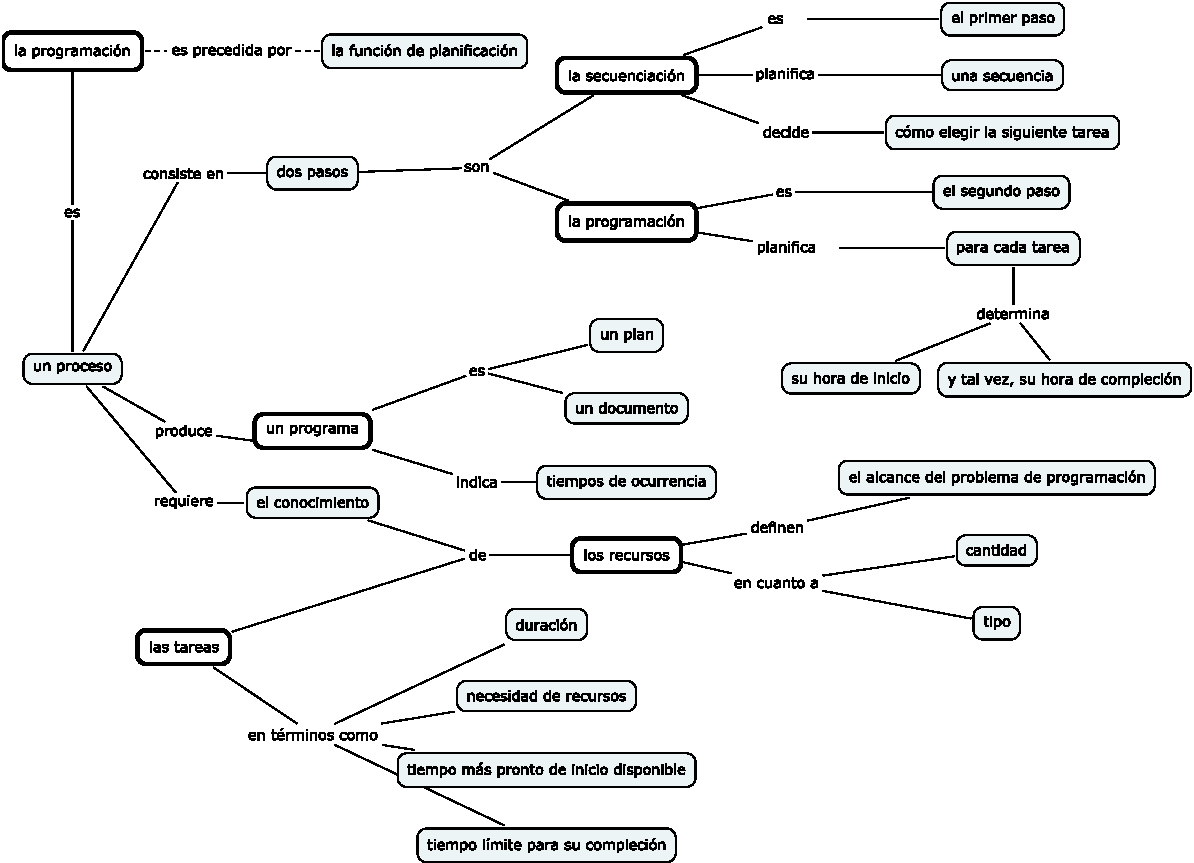
\includegraphics[width=\textheight]{scheduling.pdf}
\caption[La programación y sus elementos]{La programación y sus elementos}
\label{fig:programacion}
\end{sidewaysfigure}

\subsection{Programa, secuencia, horario}
\label{programa_secuencia_horario}

En ocasiones los términos programa\index{programa} (\textit{schedule}), secuencia\index{secuencia} (\textit{sequence}) y horario\index{horario} (\textit{timetable}) son utilizados a la ligera como si fueran sinónimos. Aquí se presentan algunas distinciones ajustándose a las prácticas aceptadas y procurando mantener tanta coherencia como sea posible.

Un \textbf{horario}\index{horario} muestra cuándo deben ocurrir eventos\index{evento} particulares. No necesariamente implica una asignación\index{asignación} de recursos\index{recursos}. Por ende, un horario publicado de trenes o autobuses muestra cuándo deben ocurrir las salidas para una o más rutas distintas, sin embargo, no nos dice cuáles vehículos o conductores han de ser asignados a trayectos en específico.
%
La asignación de vehículos y conductores es parte del proceso\index{programación!proceso} de programación. Aunque la calendarización\index{calendarización} (\textit{timetabling}) –la acción de producir horarios– es estrictamente el diseño del patrón\index{programación!patrón} de trayectos, este patrón puede ser concebido como parte de un proceso que toma en consideración si es probable que un programa\index{programa} eficiente pueda ser ajustado al patrón de trayectos resultante \cite[p.~48]{wren95scheduling-timetabling}.

En el ámbito ferroviario, el término calendarización\index{calendarización} es utilizado con frecuencia para referirse a la construcción de una ruta –con tiempos– para un tren a través de un sistema. Siendo así que el «Escocés Volador» –mundialmente famoso tren exprés de pasajeros que recorre desde 1862 el trayecto Londres-Edinburgo– solía partir de Edinburgo (estación \textit{Waverly}) a las 10:00; el trabajo de calendarización era el proceso de la búsqueda de tiempos y rutas a través del sistema de trenes que no conflictuaran con otro tráfico –haciendo revisiones en el resto del tráfico de ser necesario– hasta que llegaba a Londres (estación \textit{Kings Cross}) a las 18:30 (en 1922) o 18:05 (1948) 
\citep[p.~48, 49]{wren95scheduling-timetabling}.

Un horario\index{horario!educacional} educacional también muestra cuándo deben ocurrir eventos en particular. En ciertas circunstancias puede no haber actividad de programación\index{programación} necesaria para producir tal horario\index{horario}. En una escuela donde un único maestro es el responsable por todas las actividades\index{actividad} de una clase\index{clase} en particular, y donde dichas actividades\index{actividad} ocurren en un mismo lugar, un horario\index{horario} no es más que una declaración respecto a los tiempos en que deberán ocurrir actividades específicas –como en el caso del «Escocés Volador»–.
%
En contraste, un horario de exámenes para una universidad normalmente incluirá la asignación de aulas conociendo el tamaño de los grupos y de las instalaciones especiales requeridas. Habrá sido conformado sujeto a restricciones duras\index{restricción!dura} y suaves\index{restricción!suave}, como la cantidad de exámenes que puede presentar un estudiante en periodos consecutivos. Un horario de cursos para una universidad también tiene que tomar en cuenta la disponibilidad de los conferenciantes individualmente.
%
Es por ello que las actividades de calendarización de cursos\index{calendarización!de cursos} y calendarización de exámenes\index{calendarización!de exámenes} en universidades\index{horario!en universidades} pueden ser consideradas actividades\index{actividad} de programación\index{programación} \citep[p.~49]{wren95scheduling-timetabling}. 

Una \textbf{secuencia}\index{secuenciación!secuencia} es simplemente un orden en que las actividades\index{actividad} son llevadas a cabo. Por ejemplo, el orden en el que los trabajos son procesados a través de las máquinas en una fábrica, si los trabajos pasan a través de cada máquina en el mismo orden, es una secuencia. La secuenciación\index{secuenciación} puede tomar en cuenta costos relacionados a un trabajo específico siendo seguido por otro, como el costo de conversión de máquina. El problema de la secuenciación\index{secuenciación} de trabajos en estas circunstancias es conocido como un problema \textit{flow-shop}\index{secuenciación!flow-shop} \citep[p.~49]{wren95scheduling-timetabling}. 

Un \textbf{programa}\index{programa} normalmente incluirá toda la información espacial y temporal necesaria para que un proceso\index{proceso} llegue a término. Esto comprenderá los tiempos de inicio de las actividades\index{actividad} pertinentes, aserciones respecto a dónde serán asignados\index{asignación} cuáles recursos\index{recurso}, así como los planes de trabajo individuales para el personal o las máquinas.
%
Por consiguiente, la programación\index{programación} es el proceso\index{programación!proceso} de la elaboración del programa\index{programa}, incluyendo la asignación\index{asignación} de recursos\index{recurso} \citep[p.~49]{wren95scheduling-timetabling}.
%
En la figura \ref{fig:programa_secuencia_horario} se ilustran los conceptos anteriores.

\begin{sidewaysfigure}
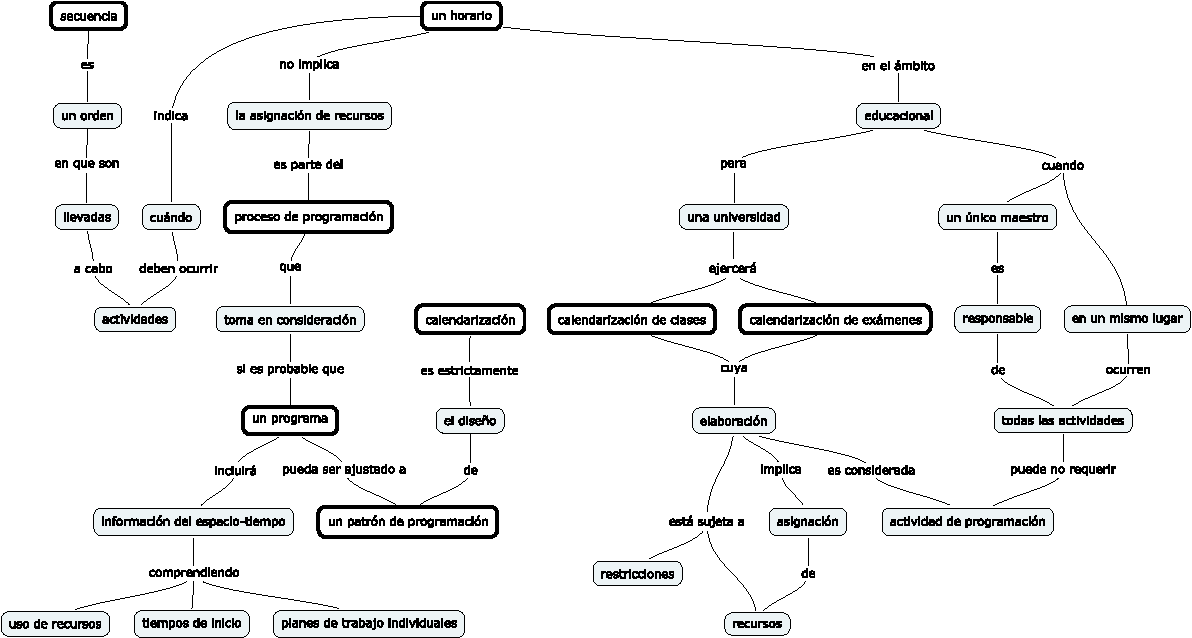
\includegraphics[width=\textwidth]{media/programa_secuencia_horario.pdf}
\caption[Programa, secuencia, horario]{Programa, secuencia, horario}
\label{fig:programa_secuencia_horario}
\end{sidewaysfigure}

\subsection{El proceso de programación} % (fold)
\label{proceso_programacion}

De acuerdo a \citet{wren95scheduling-timetabling}, \textbf{el objetivo de la programación} es solucionar problemas prácticos relacionados a la asignación, sujeta a restricciones, de recursos a objetos siendo colocados en el espacio-tiempo, haciendo uso o desarrollando herramientas apropiadas. Los problemas con frecuencia buscarán la satisfacción de ciertos objetivos \citetext{p.~47}.

\citet{wren95scheduling-timetabling} prosigue mencionando que la programación\index{programación} puede ser vista como el acomodo de recursos dentro de un \textbf{patrón\index{programación!patrón} en el tiempo o espacio} de manera tal que algunos objetivos\index{objetivo} sean alcanzados –o se acerquen a ello– y que restricciones\index{restricción} existentes en la manera en que los recursos pueden ser acomodados sean satisfechas –o casi satisfechas–.
%
Los \textbf{recursos} pueden ser personas, vehículos, clases, exámenes, máquinas, trabajos en una fábrica, es decir, cualquier cosa que sea del interés del dueño del problema.
%
Con frecuencia la conformación de los recursos puede ser vista como parte del proceso de programación\index{programación!proceso}. Por ejemplo, las herramientras de trabajo en una fábrica pueden ser acomodadas por turnos de personal, los cuales deben ser agrupados en listas, esta formación de turnos puede ser vista como un proceso específico de programación dentro de un proceso más extenso \citetext{p.~48}.

El \textbf{patrón de programación}\index{programación!patrón} puede ser un orden de eventos, una estructura de rutas, una matriz de asignaciones, entre otros. El \textbf{patrón general de programación} puede tener que ser elaborado como parte del proceso de programación, o puede ser una plantilla\index{programación!plantilla} pre-existente característica del problema\index{programación!problema general} en cuestión \citep[p.~48]{wren95scheduling-timetabling}.

Las \textbf{restricciones}\index{restricción} definen conexiones físicas o permisibles entre los recursos\index{recurso}, y entre estos y el patrón\index{programación!patrón} de programación. Ellas gobiernan la manera en la cual los recursos pueden acomodarse juntos o dentro del patrón. Las restricciones pueden ser vistas como reglas que obstaculizan el logro de los objetivos\index{objetivo}. No obstante, también pueden ser vistas como parte de la especificación del problema\index{programación!problema general} siendo posible utilizarlas para guiar a la herramienta\index{programación!herramienta} de búsqueda de soluciones a una respuesta.
%
En la figura \ref{fig:scheduling_process} se presentan los conceptos ya descritos.
%
Algunas restricciones existen únicamente desde el punto de vista del dueño del problema y pueden formar parte del proceso\index{programación!proceso} de solución, con el propósito de mostrar hasta qué grado una solución podría ser mejorada si una restricción o restricciones fueran relajadas; de manera que el dueño pueda decidir si la restricción es realmente necesaria o si vale la pena hacer el esfuerzo de eliminarla de la definición del problema \citep[p.~48]{wren95scheduling-timetabling}.

\begin{figure}[hbtp]
\centering
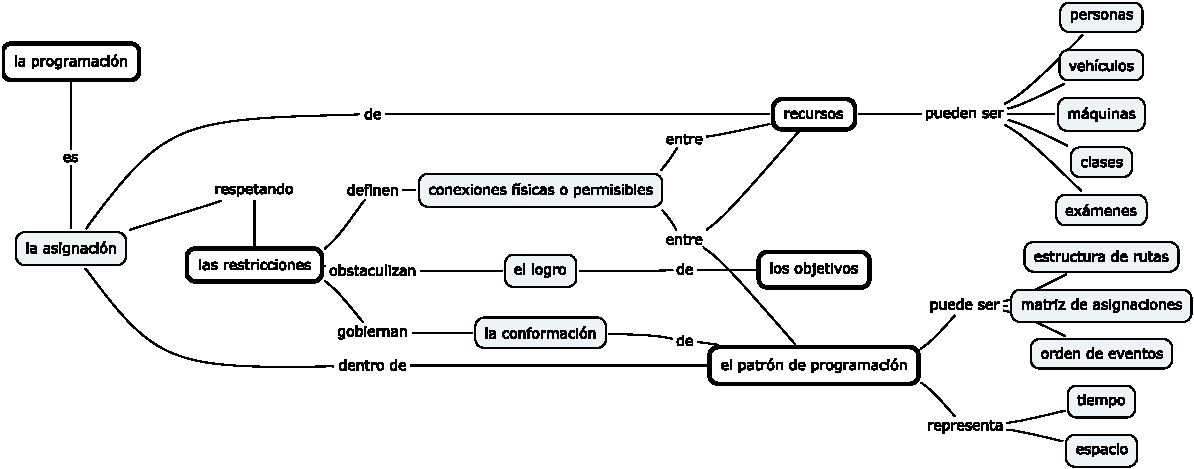
\includegraphics[width=\textwidth]{media/scheduling_process.pdf}
\caption[El proceso de programación]{El proceso de programación}
\label{fig:scheduling_process}
\end{figure}

\subsection{Definiciones}
\label{Definiciones}

Para \citet[p.~5]{TKindt2002} los problemas de programación se encuentran en todo tipo de sistemas puesto que es necesaria para la organización y/o distribución del trabajo entre múltiples entidades. En cada libro pertinente de la literatura se presenta una definición así como sus componentes principales. Una de éstas es la enunciada por \citet{carlier1988problemes}: 
\begin{quotation}
La programación es predecir el procesamiento de un trabajo al asignar recursos a tareas y fijar sus tiempos de inicio\dots Los diferentes componentes de un problema de programación son las tareas, sus restricciones potenciales, los recursos y la función objetivo\dots Las tareas deben ser programadas para optimar un objetivo específico\dots Por supuesto, frecuentemente será más realista en la práctica considerar múltiples criterios (como está citado en \citealp[p.~6]{TKindt2002}) 
\end{quotation}

Otra definición es la hecha por \citet[p.~1]{Pinedo1995}: «La programación es un proceso de toma de decisión\dots  Se encarga de la asignación de recursos a tareas durante periodos y cuya meta es la optimación de uno o más objetivos.»

Algunos autores consideran a la programación\index{programación} (\textit{scheduling}) y calendarización\index{calendarización} (\textit{timetabling}) como actividades distintas, en este trabajo se utilizará el término programación\index{programación} como un término genérico y para cubrir tipos específicos de problemas, y se considerará a la calendarización\index{programación!calendarización} (\textit{timetabling}), secuenciación\index{programación!secuenciación} (\textit{sequencing}) y establecimiento de listas\index{programación!listas} (\textit{rostering}) como casos especiales de la actividad genérica de programación\index{programación} \citep[p.~47]{wren95scheduling-timetabling}.
%
En la sub-sección \ref{proceso_programacion} se definió el objetivo de la programación como:

\begin{quotation}
solucionar problemas prácticos relacionados a la asignación, sujeta a restricciones, de recursos a objetos siendo colocados en el espacio-tiempo, haciendo uso o desarrollando herramientas apropiadas. Los problemas con frecuencia buscarán la satisfacción de ciertos objetivos.
\end{quotation}

Para \citet{wren95scheduling-timetabling}, las actividades de calendarización\index{programación!calendarización}, establecimiento de listas\index{programación!listas} y secuenciación\index{programación!secuenciación} todas se apegan a la definición anterior.
%
Sin embargo, se hará uso de las siguientes definiciones más restrictivas para este trabajo.

\begin{quotation}
La \textbf{programación} es la asignación, sujeta a restricciones, de recursos a objetos siendo colocados en el espacio-tiempo, de manera tal que se minimice el costo total de algún conjunto de los recursos usados. Ejemplos comunes son la programación de transporte o el diseño de rutas para vehículos de entrega que buscan minimizar el número de vehículos o conductores y dentro de ese mínimo de recursos, minimizar el costo total; y la programación \textit{job-shop} que puede buscar minimizar el número de periodo de tiempos usados, o algún recurso físico.

La \textbf{calendarización} es la asignación, sujeta a restricciones, de recursos dados a objetos siendo colocados en el espacio-tiempo, de manera tal que se satisfaga tanto como sea posible un conjunto de objetivos deseados. De ejemplo están la calendarización de cursos y exámenes y algunas formas de asignación de personal, como la ocupación de puestos en casetas de cobro sujetas a un número limitado de personal.

La \textbf{secuenciación} es la construcción, sujeta a restricciones, de un orden en el que determinadas actividades deben ser llevadas a cabo u objetos que deben ser colocados en alguna representación de una solución. Como ejemplos están la programación \textit{flow-shop} y el problema del agente viajero (\textit{travelling salesman problem; TSP}).

El \textbf{establecimiento de listas} es la colocación, sujeta a restricciones, de recursos en espacios dentro de un patrón. Se puede buscar alcanzar algún objetivo o simplemente lograr una asignación factible. Frecuentemente los recursos rotarán a través de una lista. \citetext{p.~53}
\end{quotation}

\begin{figure}[hbtp]
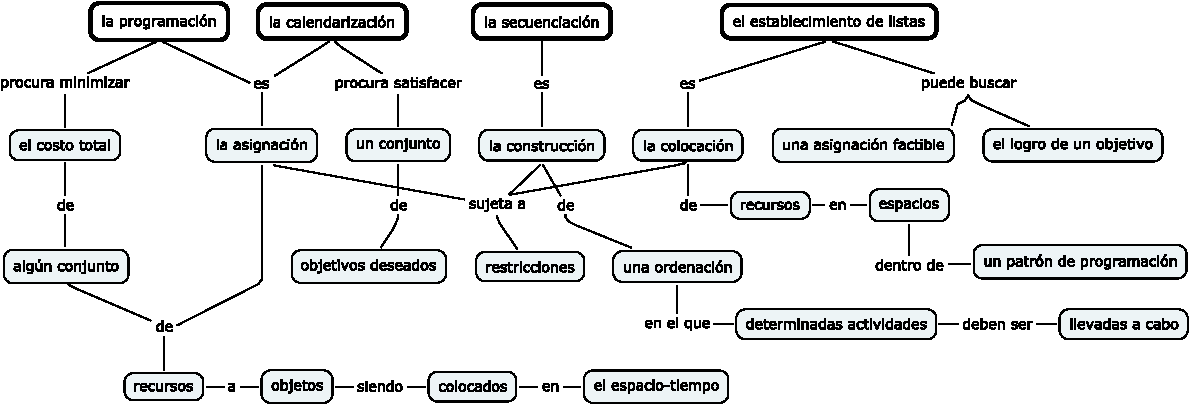
\includegraphics[width=\textwidth]{media/definiciones.pdf}
\caption[Definiciones]{La definición de programación, calendarización, secuenciación y establecimiento de listas}
\label{fig:definitions}
\end{figure}

Algunos problemas pueden encajar en más de una de las deficiones anteriores, y los términos tienen a ser utilizados de manera holgada en el área de trabajo y en la comunidad de investigación del área. En la figura \ref{fig:definitions} se puede ver una representación de lo expuesto con anterioridad.
%
En algunas definiciones se ha referido a la satisfacción o a la minimización. Debe ser resaltado que muchos de los problemas que se tratan en el área no tienen un objetivo bien definido. En ocasiones se puede justificar el uso de métodos de mejora o no-óptimos en parte porque los distintos dueños del problema tienen distintas perspectivas del objetivo, aunque en realidad tales métodos son frecuentemente utilizados simplemente porque no hay un método óptimo –o exacto– que sea viable en la práctica \citep[p.~53,~54]{wren95scheduling-timetabling}

\section{Historia}
\label{historia_programacion}

El concepto de programación no es nuevo; las pirámides tienen más de 3,000 años, Sun Tzu escribió acerca de programación y estrategia desde una perspectiva militar hace 2,500 años, vías ferroviarias han sido construidas por alrededor de 200 años, entre otros muchos ejemplos. Ninguna de estas actividades pudo haber sido lograda sin alguna forma de programación –como lo es el entendimiento de conceptos como actividad y secuenciación–. Sin embargo, mientras que los administradores, sacerdotes y líderes militares en control de las organizaciones responsables por el logro de estas actividades debieron tener una apreciación por la programación –o al menos aquellos que tuvieron éxito– existe poca evidencia de procesos formales hasta la aparición del siglo XX \citep[p.~2]{Weaver2006}.

\begin{figure}[hbtp]
\centering
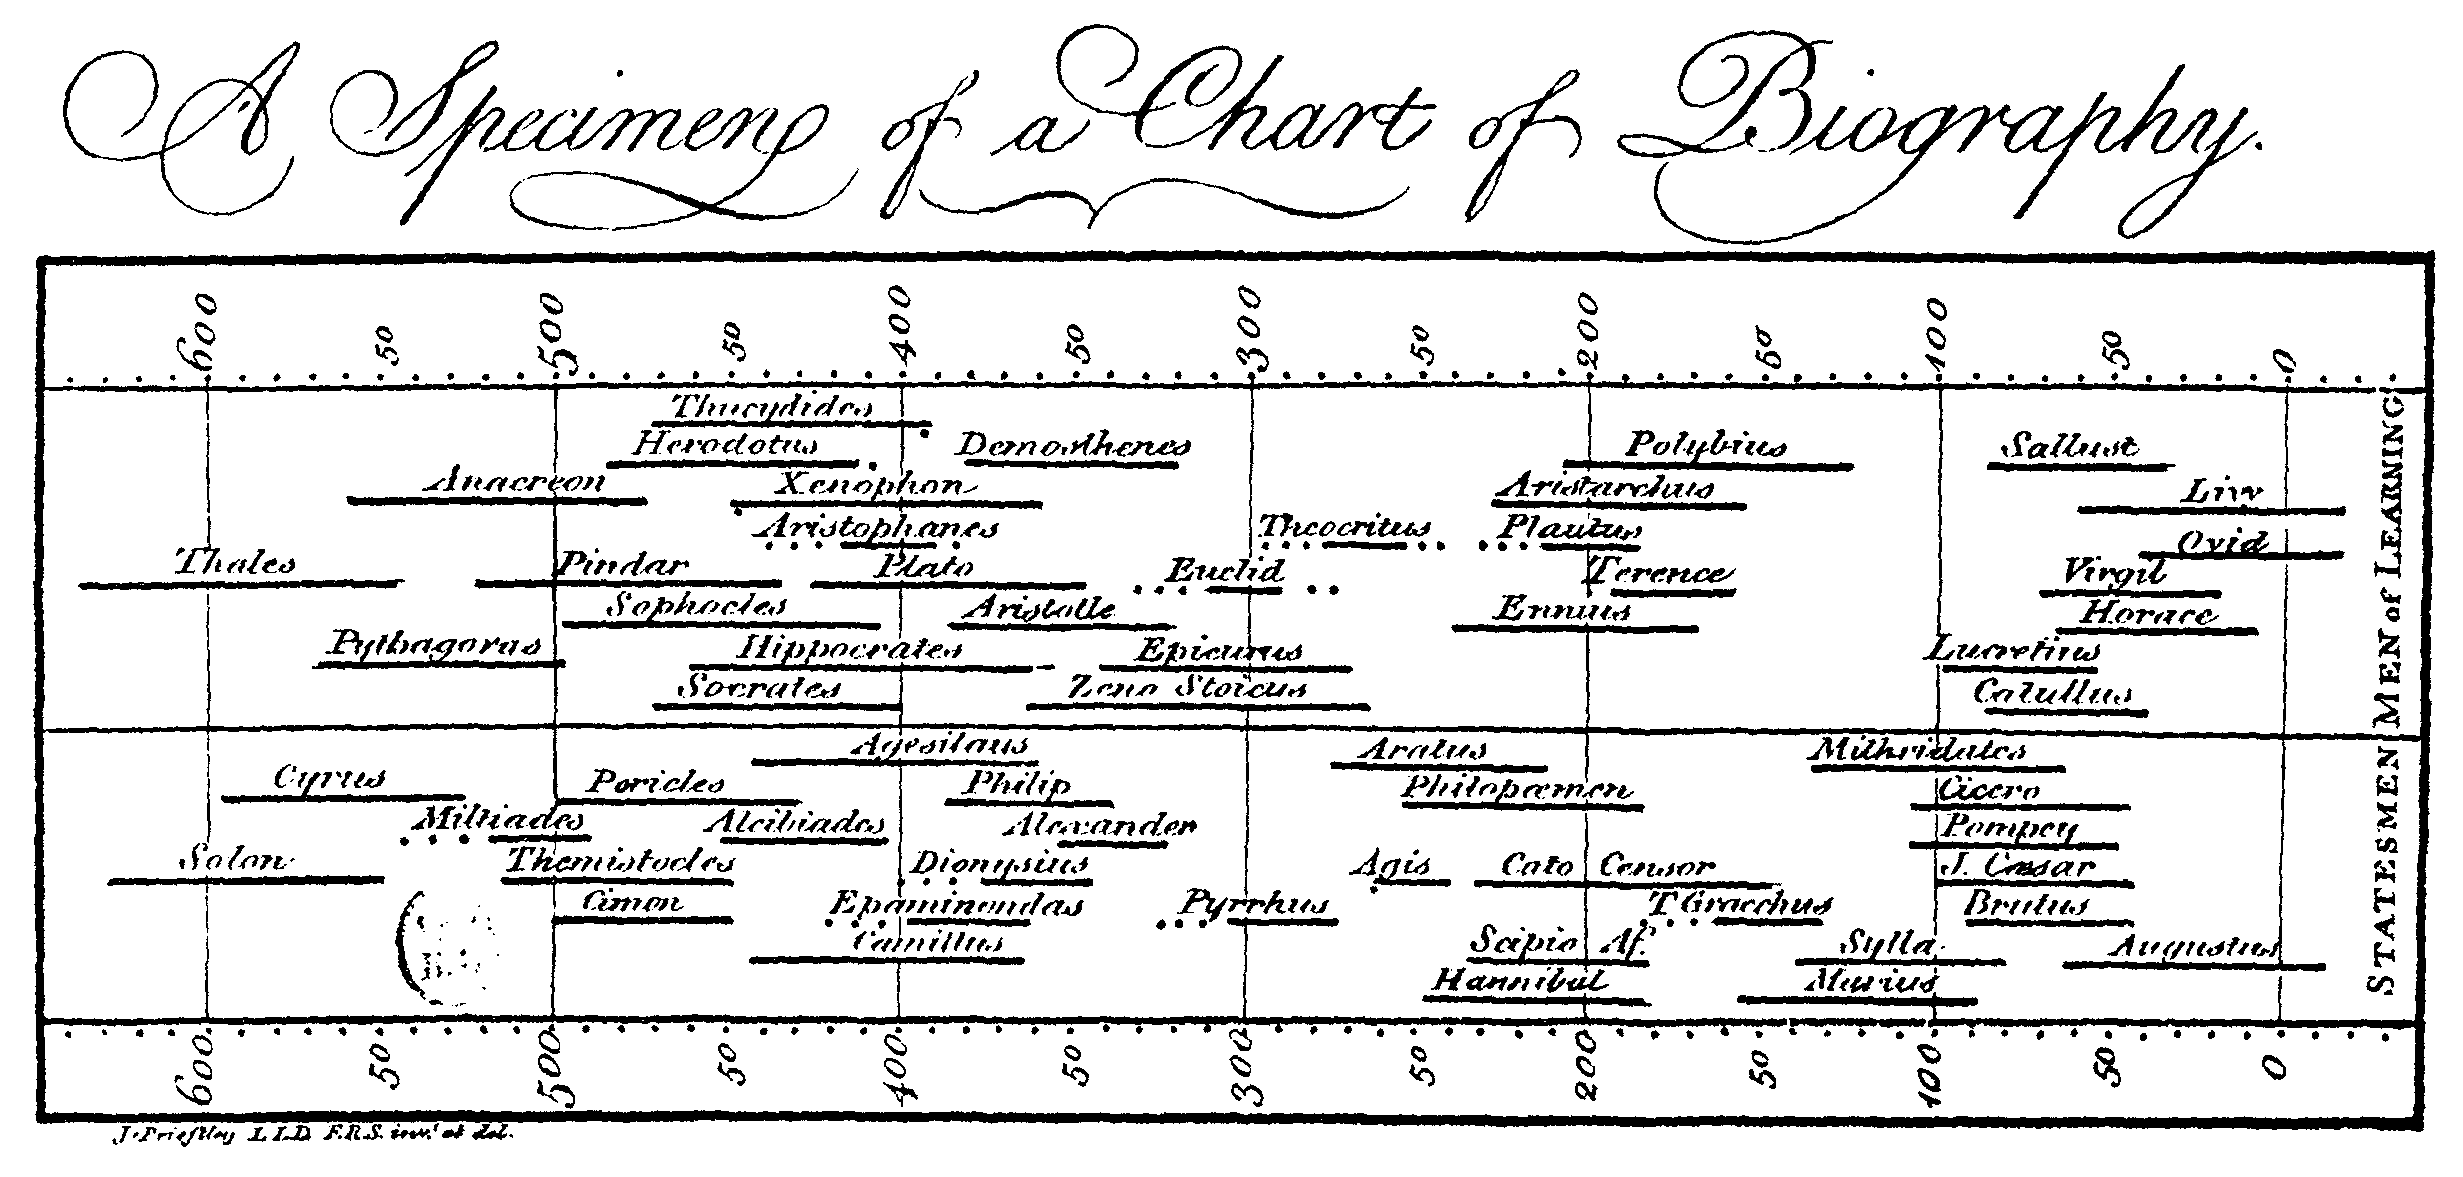
\includegraphics[width=.8\textwidth]{media/PriestleyChart.png}
\caption[Gr\'afica de Biograf\'ia]{Gr\'afica de Biograf\'ia abarcando los primeros 650 años antes de la era común. De \textit{A description of a chart of biography}, por J. \citeauthor{priestley1764description}, \citeyear{priestley1764description}. Derechos de autor expirados, obra del dominio público.}
\label{fig:chart_biography}
\end{figure}

De acuerdo a \citet{Weaver2006}, las herramientas de control de programación modernas pueden trazar sus orígenes hasta 1765. El creador de la «gráfica de barra» (\textit{bar chart}) parece ser Joseph Priestley (Inglaterra, 1733-1804); su «Gráfica de Biografía» (\textit{Chart of Biography}) mostraba unos 2,000 lapsos de vida de personajes notables en una gráfica con escala de tiempo, véase la figura \ref{fig:chart_biography}. Las ideas de Priestley fueron retomadas por William Playfair (1759-1823) en su «Atlas Comercial y Político» (\textit{Commercial and Political Atlas}) de 1786. A Playfair se le atribuye el desarrollo de un vasto rango de gráficas incluyendo la línea, la barra (histograma), y las gráficas circulares (gráficas de pastel), un ejemplo puede ser visto en la figura \ref{fig:playfair_timeseries} \citetext{p.~2,~3}.

\begin{sidewaysfigure}
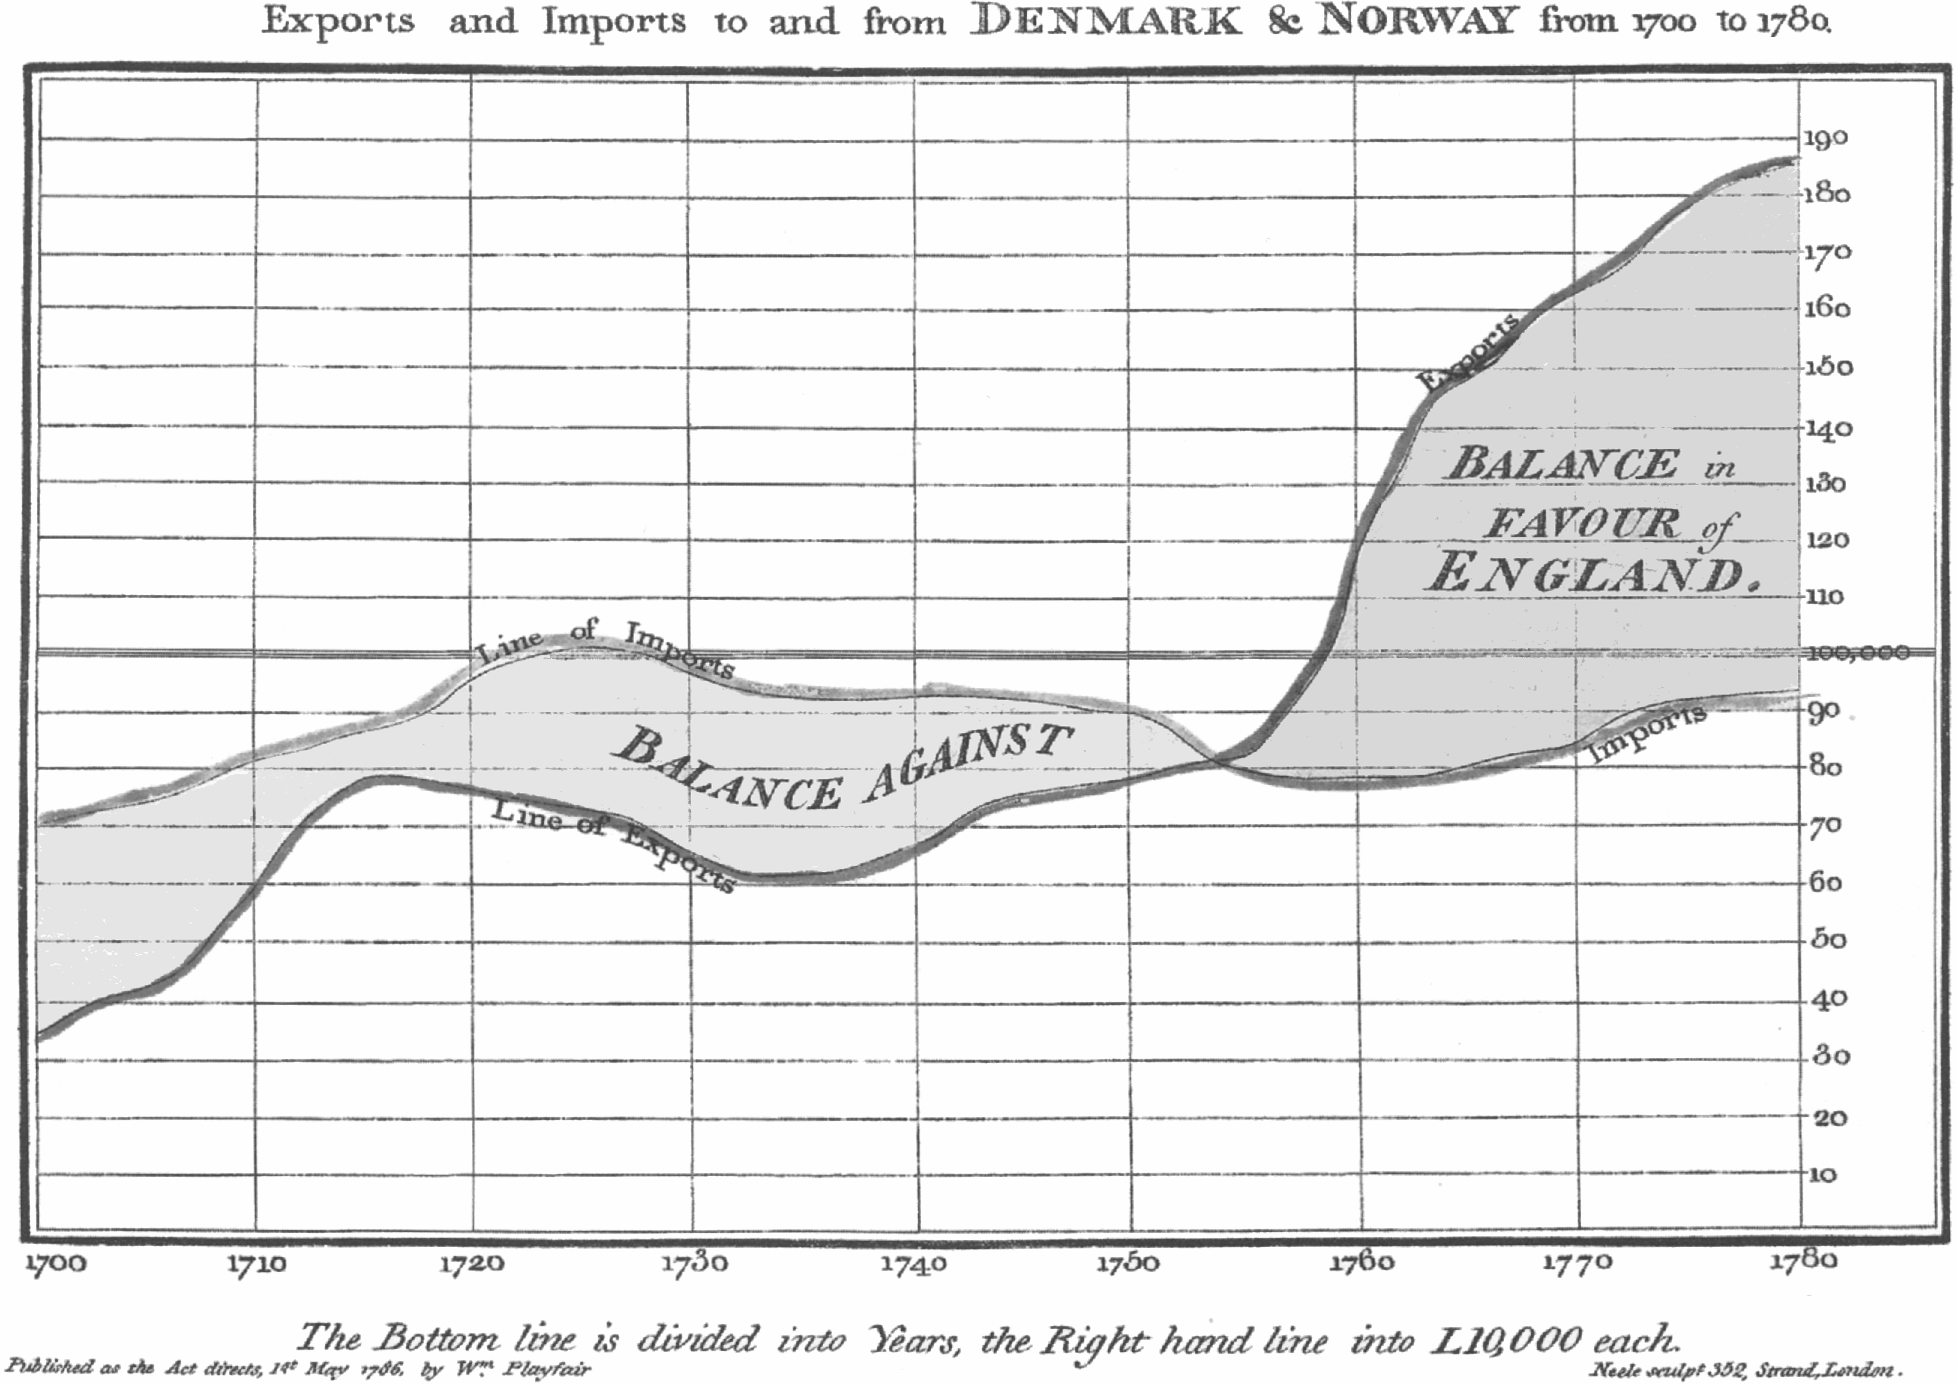
\includegraphics[width=\textwidth]{media/Playfair_TimeSeries.png}
\caption[Gráfica del Atlas de W. Playfair]{Una de las gráficas elaboradas por Playfair. De \textit{The Commercial and Political Atlas}, por W. \citeauthor{playfair1786commercial}, \citeyear{playfair1786commercial}. Derechos de autor expirados, obra del dominio público.}
\label{fig:playfair_timeseries}
\end{sidewaysfigure}

\citet{Weaver2006} recuenta que siguiendo los pasos de Playfair, Karol Adamiecki –un polaco economista, ingeniero e investigador de la administración– desarrolló el harmonograma (\textit{Harmonogram}) en 1896. Este gráfico dispone de una escala de tiempo en el eje  vertical (en el lado izquierdo) y enumera las actividades en la parte superior. La hora de inicio y la duración de las actividades se muestra por una «barra deslizante» (\textit{sliding tab}), muy similar a la «barra» en una gráfica de barra. Lo relevante del harmonigrafo (\textit{Harmonygraph}) es que también tabula para cada actividad sus predecesores y sucesores haciéndolo un predecesor destacado de los sistemas \textit{CPM} y \textit{PERT} desarrollados unos 60 años después \citetext{p.~3}.

Para 1912, la gráfica de barras moderna parece estar totalmente desarrollada y es utilizada al menos en Alemania. Estas ideas fueron entonces divulgadas en EEUU por el consultor de administración estadounidense Henry L. Gantt, quien publicó «Trabajo, Sueldos y Utilidades» (\textit{Work, Wages, and Profits}) en 1916 en donde expresamente habla de la programación, especialmente en el entorno de los talleres de trabajo. En su forma más pura, la gráfica de barras correlaciona actividades y tiempos en una presentación gráfica permitiendo la determinación de la temporización del trabajo pero no de sus interdependencias. Como se muestra en la figura \ref{fig:grafica_gantt}, la secuenciación es inferida en lugar de ser mostrada y en sus elaboraciones hechas a mano, las primeras gráficas eran una representación estática del programa \citep[p.~3]{Weaver2006}.

\begin{sidewaysfigure}
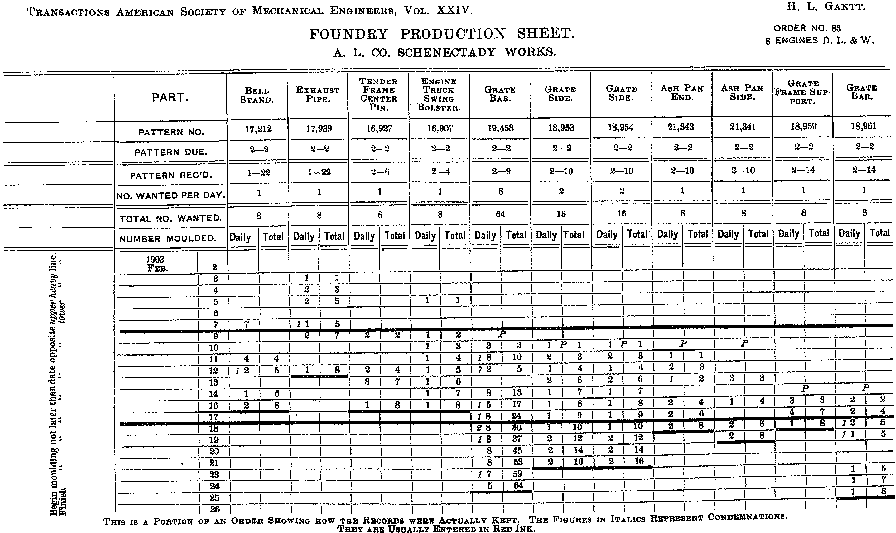
\includegraphics[width=\textwidth]{media/gantt-graphic.pdf}
\caption[Gráfica de Gantt]{Gráfica de Gantt. De \textit{Gantt charts: A centenary appreciation}, por J. M. \citeauthor{wilson2003gantt}, \citeyear{wilson2003gantt}, \textit{European Journal of Operational Research}, 149, p.~2. Derechos reservados [\citeyear{wilson2003gantt}] por \textit{European Journal of Operational Research}.}
\label{fig:grafica_gantt}
\end{sidewaysfigure}

La planeación de líneas de flujo (\textit{flowline planning}) fue desarrollada en la década de los treinta o aún antes y las gráficas de hitos (\textit{milestone chart}) también estuvieron en uso regular para la década de los cincuenta. Grandes contratos eran subdivididos en secciones con fechas límite de compleción del trabajo necesario para lograr cada hito (\textit{milestone}). Sin embargo, así como con las graficas de Gantt, todas las fechas y las relaciones mostradas en estas graficas estaban basadas en heurísticas o en experiencia. Era posible identificar retrasos pero cualquier valoración del impacto del mismo estaba basada en una interpretación personal de los datos y no de un análisis serio. Como consecuencia cuando el retraso de un programa se volvía aparente en grandes contratos, la tendencia era solucionar el problema inundándolo con mano de obra y «comprar tiempo» frecuentemente a un precio muy elevado.
%
Independiente del desarrollo de los procesos de control de programación basados en gráficas de barras y de hitos, la programación lineal había estado siendo investigada durante varios años. Esta rama de las matemáticas observaba las dinámicas de causa y efecto de acciones entre ellas mismas, en situaciones tales como el flujo de tráfico en una autopista. Uno los matemáticos involucrados en este trabajo fue James E. Kelley \citep[p.~4]{Weaver2006}.

\subsection{Método de la ruta crítica} % (fold)
\label{sub:Metodo_ruta_critica}

El origen del método de la ruta crítica (\textit{Critical Path Method; CPM}) data de mediados de 1956. La empresa Du Pont estaba en búsqueda de problemas que pudiera solucionar a través de su computadora «UNIVAC1» –una de las primeras computadoras instaladas en el ámbito comercial–. La administración de Du Pont acordó que el estudio de la planeación, estimación y programación sería un buen uso de la computadora. La encomienda de descubrir si una computadora podría ser programada para ayudar le fue otorgada a Morgan Walker. Muchos otros habían comenzado a estudiar el problema, incluso colegas de Du Pont pero ninguno había logrado un fin económicamente viable \citep[p.~4,~5]{Weaver2006}.

En el periodo desde fines de 1956 hasta abril de 1957, Walker con la asistencia de Kelly y otros había examinado un proyecto viable. El reto era solucionar el dilema del tiempo-costo. Podían demostrar que en lugar inundar un proyecto retrasado con mano de obra para recuperar tiempo perdido, enfocar el esfuerzo en las tareas «correctas» podía reducir el tiempo de compleción sin aumentar el costo de manera significante. El problema estriba en encontrar cuáles son las tareas «correctas» \citep[p.~5]{Weaver2006}.

El equipo de Du Pont era liderado por Morgan R. Walker, participantes clave provenientes del equipo Univac fueron James E. Kelley y John Mauchly. Kelley era el experto en matemáticas y cómputadoras nominado por Mauchly para solucionar el problema para Walker. La solución adoptada por Kelley estaba basada en la programación lineal y utilizaba la notación matemática de subíndices para describir la relación entre actividades. Esto limitaba la secuenciación y hacía posible que el cómputo fuera factible.
%
La solución creaba un par de retos significantes. Uno era la recopilación de los datos necesarios para cargar el modelo computacional. Los ingenieros no estaban acostumbrados a describir trabajo en términos de actividades (tareas) con requerimientos de recursos y distintos costos dependiendo de los recursos empleados para una duración «normal» y una duración «en crisis». La recopilación de los datos para el primer modelo \textit{CPM} le tomó a Walker más de tres meses. El otro problema era que la notación de subíndices carecía de sentido salvo para los matemáticos. El diagrama de «Actividad-en-Flecha» fue desarrollado para explicar las matemáticas a los administradores. A pesar de todos los problemas, el 24 de julio de 1957 el primer análisis del programa de \textit{George Fischer Works} había sido completado y el concepto comprobado. El programa incluía 61 actividades, 8 restricciones de tiempo y 16 restricciones ficticias. Una parte del programa puede ser visto en la figura \ref{fig:cpm_george_fischer_works} \citep[p.~5,~6]{Weaver2006}.

\begin{sidewaysfigure}
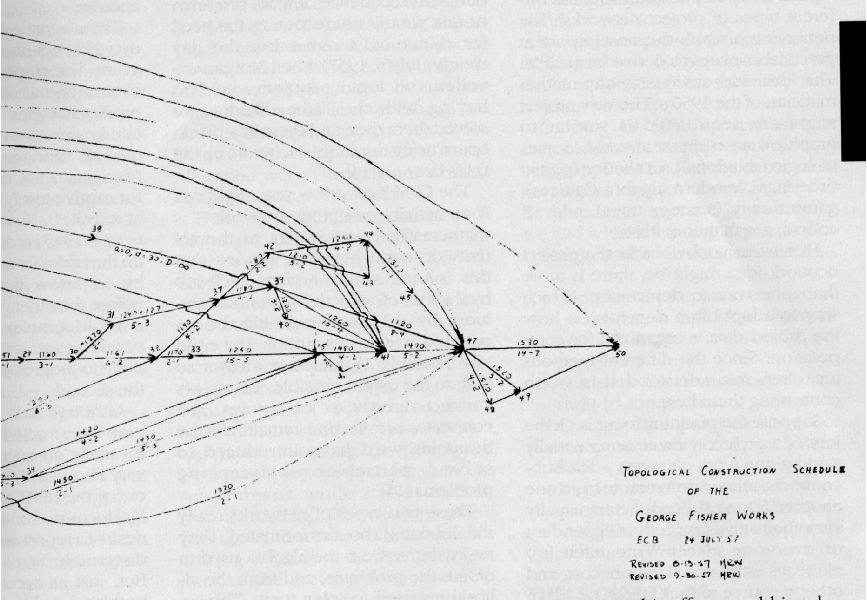
\includegraphics[width=\textwidth]{media/cpm_gfw.pdf}
\caption[Gráfica de CPM]{Una sección del programa \textit{CPM} de \textit{George Fischer Works}. De \textit{A Brief History of Scheduling}, por P. \citeauthor{Weaver2006}, \citeyear{Weaver2006}, p.~6. Derechos reservados [\citeyear{Weaver2006}] por \textit{Mosaic Proyect Services Pty Ltd}.}
\label{fig:cpm_george_fischer_works}
\end{sidewaysfigure}

El mayor reto luego se convirtió en reducir el número de cálculos y variables a un nivel que pudiera ser procesado en un tiempo razonable. El estimado del tiempo necesario para actualizar un programa de 150 a 300 flechas era de alrederdor de 350 horas de tiempo de computadora al mes. Algunos de los retos eran básicos: como tener acceso a la computadora adecuada; las cintas magnéticas con la información almacenada eran preparadas en las computadoras de Du Pont y después trasladadas atravesando EEUU para ser ejecutadas en máquinas capaces de analizar los datos. El desarrollo continuó todo 1958 y en marzo de 1959 Kelley y Walker de manera conjunta, presentaron \textit{CPM} al público en general en la Conferencia de Computadoras del Este Unido (\textit{Eastern Joint Computer Conference}) en un artículo llamado «Planificación y Programación de la Ruta Crítica» (\textit{Critical Path Planning and Scheduling}) \citep[p.~6]{Weaver2006}.

% subsection Método de la ruta crítica (end)

\subsection{Técnica de revisión y evaluación de programas} % (fold)
\label{sub:pert}

La Técnica de Revisión y Evaluación de Programas (\textit{Program Evaluation and Review Technique; PERT}) fue desarrollada por la Oficina de Proyectos Especiales de la Marina de los EEUU. Introdujo la incertidumbre a las duraciones del programa, pero la contribución más importante que hizo el equipo de \textit{PERT} a la programación fue la invención de la «ruta crítica» (\textit{critical path}). Kelly y Walker utilizaron el nombre «cadena principal» (\textit{main chain}) para la ruta más extensa a través del programa \citep[p.~7]{Weaver2006}.

A pesar de que \textit{PERT} y \textit{CPM} surgieron independientemente, son marcadamente similares, ambos usan la técnica de diagramas de flecha –con las flechas representando actividades– y son considerados como herramientas para la planeación y programación de grandes proyectos no-repetitivos. La diferencia fundamental es que el negocio de Du Pont era bien conocido –construcción y mantenimiento de plantas químicas– y las duraciones de las actividades podían ser estimadas con cierto grado de exactitud basándose en valores históricos conocidos y tasas de producción. Consecuentemente, \textit{CPM} se enfocó en la optimación de costos al hacer balance de recursos. El trabajo de la Marina fue meramente de investigación y desarrollo, contemplando el costo como un factor secundario; las duraciones solo podían estimarse y \textit{PERT} se enfocó en la determinación de la probabilidad de ocurrencia de un evento en una fecha futura. Sin embargo, su utilidad potencial tiene un alcance mucho más amplio. Ambos han ganado una rápida aceptación como útiles técnicas prácticas y han sido empleados exitosamente en diversas áreas, incluyendo investigación y desarrollo, construcción, manutención, mercadotecnia y producción. Para fines de la década de los sesenta tanto \textit{CPM} como \textit{PERT} se fusionaron en sistemas de administración basados en red \citep[p.~372,~8]{Baker2009,Weaver2006}.

% subsection Técnica de revisión y evaluación de programas (end)
\subsection{Desarrollo en otras partes del mundo} % (fold)
\label{sub:desarrollo_otras_partes_mundo}

El desarrollo de sistemas de programación no estuvo basado exclusivamente en EEUU. En Europa fueron desarrollados un número de sistemas aunque ninguno sobrevivió como herramienta preponderante. Para 1968 \textit{PERT} y \textit{CPM} habían emergido como las nomenclaturas estándar y los sistemas dominantes.

En el Reino Unido la compañía química ICI pudo haber desarrollado una herramienta tipo \textit{CPM} tan pronto como 1955 en sus instalaciones de Billingam. La programación del mantenimiento de la planta era realizado a través de la «duración de secuencia controlada» de ICI haciendo uso de datos de \textit{Work Study} para estimar las duraciones y una «red de secuenciación», desafortunadamente, poca información se ha encontrado respecto a este sistema. 
%
La Sección de Investigación de Operaciones (\textit{Operational Research Section; ORS}) del Consejo Central para la Generación de Electricidad (\textit{Central Electricity Generating Board; CEGB}) en los años 1957 y 1958 estuvieron involucrados en el desarrollo de su versión de \textit{CPM}. Al seguir desarrollando su método tipo \textit{CPM} y al aplicarlo al apagado y mantenimiento de la central eléctrica Keadby en Leicestershire en 1957, el \textit{CEGB} fue capaz de reducir el tiempo de apagado en un 42\% en comparación al promedio de años anteriores, y en 1960 alcanzó a mejorar la reducción en otro 32\%. Desafortunadamente estos sucesos no fueron ampliamente publicitados y cayeron en el olvido. Es posible que una parte significativa del trabajo de \textit{ORS-CEGB} haya sido integrado –o cuando menos influenciado– en los antepasados de la compañia ICL en el desarrollo de lo que se convirtió su software de programación para \textit{mainframe} «ICL PERT», así como sus sucesores para sistemas \textit{PC} como Micro Planner y PlanTrac \citep[p.~8]{Weaver2006}.

La URSS (Rusia) desarrolló su propio sistema tipo \textit{PERT} llamado \textit{Setevoe planirovanie i upravlenie}. Si bien no tuvo un impacto fuera de la URSS, los programadores rusos han desarrollado otras herramientas interesantes, una de las más recientes es el Proyecto ARAÑA (\textit{Project SPIDER}) –véase figura \ref{fig:screenshot_project_spider}– que enlaza dinámicamente tiempo, recursos y costo –el objetivo original del trabajo de Kelley y Walker– dentro de un perfil de riesgo controlado \citep[p.~8]{Weaver2006}.

\begin{sidewaysfigure}
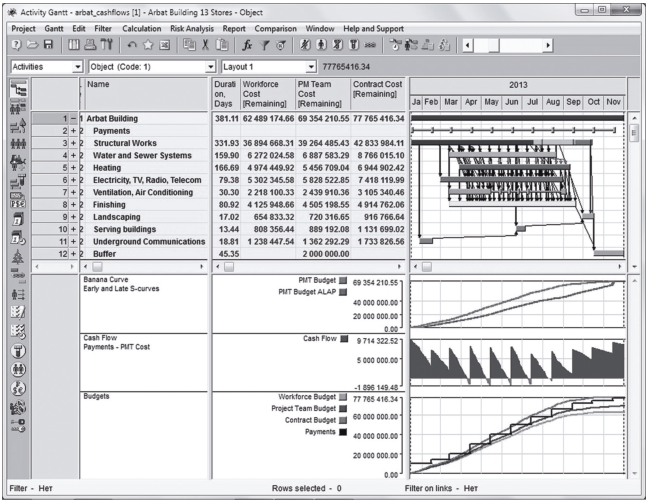
\includegraphics[width=\textwidth]{media/spider_project_gray.pdf}
\caption[Interfaz del Proyecto ARAÑA]{Una captura de pantalla de la herramienta rusa de programación «Proyecto ARAÑA». De \textit{Spider Project Professional}, por P. \citeauthor{cotterell14spider-project}, \citeyear{cotterell14spider-project}, p.~2. Derechos reservados [\citeyear{cotterell14spider-project}] por \textit{Spider Project}.}
\label{fig:screenshot_project_spider}
\end{sidewaysfigure}

El método Metra Potencial (\textit{Metra Potential Method; MPM}) desarrollado en 1958 por el Sr. B. Roy con la consultoría METRA en Francia, pudo haber sido influenciado por avances en los EEUU pero parece haber sido inventado de manera independiente del trabajo del Dr. John Fondahl en el sistema de precedencias. \textit{MPM} empleaba un sistema gráfico de «nudos» –puntos y círculos– unidos por «tiras». Las «tiras» –líneas entre los nudos– podían o no tener una dirección de flujo pero sí especificaban el periodo de tiempo que una actividad estaba indicada a demorarse después del inicio de la actividad predecesora. La herramienta alemana «ACOS Plus 1» utiliza \textit{MPM} como su filosofía de programación aunque desde una perspectiva de usuario, \textit{ACOS} es similar a la mayoría de las herramientas de programación basadas en precedencia. Sin embargo, ACOS ofrece un número adicional de tipos de enlaces. \textit{MPM} fue probablemente el primer sistema en utilizar «demoras» en sus algoritmos de programación \citep[p.~8,~9]{Weaver2006}.

% subsection Desarrollo en otras partes del mundo (end)

\subsection{El método de diagramación de precedencias} % (fold)
\label{sub:metodo_programacion_precedencia}

En 1961 el Dr. John Fondahl publicó un reporte titulado «Un enfoque no-computarizado hacia métodos de ruta crítica para la industria de la construcción» (\textit{A Non-computer Approach to Critical Path Methods for the Construction Industry}). Este documento describió al sistema de programación \textit{PDM} (\textit{Precedence Diagramming Method}) y fue presentado como un proceso manual efectivo para evitar el uso del oneroso sistema basado en ordenadores \textit{CPM}.
%
El planteamiento desarrollado por el Dr. Fondahl hacia uso de un diagrama elaborado a partir de «círculos y línea conectoras» (\textit{circle and connecting lines}) derivado de los diagramas de flujo de procesos o gráficas de flujo –tanto \textit{CPM} como \textit{PERT} utilizaban la notación de Actividad-en-Flecha–. Algunos de los enfoques clave del planteamiento fueron:

\begin{itemize}
\item El impacto del intercambio tiempo/costo –el mismo problema que Kelley y Walker estaban trabajando–.
\item Responder a la pregunta «¿Puede el personal interno de los contratistas trabajar con \textit{CPM} sin tener acceso a ordenadores?»
\item La simplicidad percibida al hacer uso de gráficas de flujo.
\end{itemize}

A pesar del énfasis en la investigación del Dr. Fondahl en la no utilización de ordenadores, sus colegas en la firma Texana H.B. Zachry Co. de San Antonio comenzaron a trabajar en 1962 en la implementación del sistema como una herramienta de computación para los ordenadores centrales (\textit{Mainframes}) de IBM y al menos uno de los estudiantes del Dr. Fondahl, Dick Bryan (Stanford 1955) trabajó para Zachry, convirtiéndose en vice-presidente más tarde \citep[p.~9]{Weaver2006}.

El trabajo en Stanford continuó independientemente del proyecto de Zachry e incluyó el desarrollo de un proceso de actualización manual. Este reporte –Reporte Técnico No. 47– fue publicado en 1964 y causó una re-evaluación del nombre dado a este método. Los nombres en uso durante ese periodo para el método incluían «círculo-y-línea-conectora» (\textit{circle-and-connecting-line}), «operación y línea de interrelación» (\textit{operation and interrelation line}) y «Actividad-en-Nodo» (\textit{Activity-on-Node}) propuesto por Moder y Phillips en la primera edición de su libro «Administración de Proyectos con \textit{CPM} y \textit{PERT}» (\textit{Project Management with CPM and PERT}) publicado en 1964. Sin embargo, a comienzos de 1964 IBM anunció el lanzamiento de su «Sistema de Control de Proyectos» (\textit{Project Control System; PCS}) para la computadora 1440. \textit{PCS} utilizó el nombre «diagramación de precedencias» (\textit{precedence diagramming}) y el equipo de Stanford decidió adoptar el mismo nombre pues dado el uso de IBM, éste probablemente prevalecería \citep[p.~9]{Weaver2006}.

La transición del trabajo del Dr. Fondahl a un sistema basado en computadora parece haber sido diseñado por la compañía Texana de construcción Zachry. En 1958 el Sr. Zachry se hizo de un nuevo libro, «Investigación de Operaciones» (\textit{Operations Research}), y se lo dio a W.D. Tiner, Jr. –el Director de investigación en la firma– solicitándole su estudio y aplicación de sus métodos dentro de la compañía. Después de un estudio minucioso de los métodos y costos potenciales para el equipo de computación necesario, Tiner le comentó a Zachry que la compañía no podía solventar tal cantidad de dinero en los equipos. La respuesta de Zachry fue: «Doug, estás equivocado, no podemos no invertir en esos equipos».
%
La compañía Zachry comenzó a experimentar con el método de la ruta crítica (\textit{CPM}) en la programación de proyectos de construcción en 1959. Algunos de los primeros proyectos en beneficiarse de esta iniciativa incluyeron la construcción de una base de misiles Atlas en Abilene, Texas en 1960 haciendo uso de tiempo rentado en una IBM 650 y la construcción de una nueva instalación para Nike Zeus en la isla Kwajalein (en las Islas de Marshall) en 1961 haciendo uso de una computadora IBM 1620 instalada en las oficinas de Zachry \citep[p.~9,~10]{Weaver2006}.

% subsection El Método de Diagramación de Precedencias (end)

\subsection{La programación y la computadora} % (fold)
\label{sub:programacion_computadora}

La evolución de la programación siguió de cerca el desarrollo de las computadoras. Los primeros sistemas eran computadoras centrales gigantescas, típicamente le tomaba a un nuevo programador muchos meses aprender a utilizarlas. Estos sistemas migraron a las mini-computadoras de la década de los setenta y ochenta pero continuaron siendo onerosos, fomentando así el uso generalizado de técnicas manuales de programación, solo las organizaciones más grandes –o más sofisticadas– pudieron sufragar una oficina central de programación y los sistemas de cómputo necesarios. 
%
El advenimiento de la micro-computadora –entiéndase la \textit{PC} o computadora personal– cambió la programación para siempre. La evolución de la programación basada en tecnología \textit{PC} cambió los controles del proyecto, de un ambiente en donde un equipo especializado de programadores operaba sistemas costosos asegurándose que la programación fuera correcta –y que la organización tuviera el control de los datos– a una situación en donde cualquiera podía aprender a manejar un paquete de software de programación; los programas se convirtieron en «islas de información» dispersas en los escritorios de los empleados y la calidad de la programación en general se desplomó \citep[p.~2]{Weaver2006}.

En la actualidad, hay tendencias de un regreso a los sistemas empresariales soportados por paquetes Ofimáticos de Administración de Proyectos (\textit{Project Management Office; PMO}) que remedian el equilibrio y ofrecen lo mejor de los dos mundos. Desde un punto de vista tecnológico, la información es gestionada de manera central, pero está disponible fácilmente para todos en cualquier \textit{PC} a través de una interfaz de red. Desde el punto de vista de habilidades, los \textit{PMO} están teniendo un impacto en el desarrollo de las carreras de los programadores y apoyando en la implementación de estándares de programación dentro de las organizaciones \citep[p.~2]{Weaver2006}.

Antes de la década de los ochenta la programación era considerado un asunto muy serio; hacía uso de recursos costosos, requería de significante entrenamiento y habilidad, y estaba mayormente centralizada y visible. En donde se hacía uso de la programación manual, los ahorros en costos de operación eran contrarrestados por el tedio de las extensas computaciones manuales; no era redituable cometer equivocaciones, por ende los programadores eran profesionales entrenados.
%
La llegada de herramientas de programación «fáciles de utilizar» con una interfaz gráfica cambió radicalmente a la industria. La programación migró al escritorio y surgió el mito de que «cualquiera» podía crear un programa –considerando que supiera encender una \textit{PC}–. Mucha gente aprendió «programación» al usar herramientas como \textit{Microsoft Project}. No había entrenamiento o supervisión y como consecuencia, el programa promedio estaba inundado de «arreglos» permitidos o incluso fomentados por la herramienta. La tendencia ha sido hacia un enfoque en los procesos computacionales y la obtención de un programa que se «vea bien» en lugar de el análisis de un proyecto para determinar la duración apropiada basada en las disponibilidades de los recursos apropiados y en el diseño de un programa como una herramienta efectiva para la administración en el contexto de cada proyecto en específico \citep[p.~12,~13]{Weaver2006}.

\chapter{Teoría de la programación}
\label{teoria_programacion}

\section{Introducción}

Muchos de los primeros desarrollos en el campo de la programación fueron motivados por problemas encontrados en la industria de la producción. Por lo tanto, es natural encontrar en la literatura el uso de vocabulario de producción cuando se describen problemas de programación. Aún cuando hoy día la aplicación de la programación es de considerable importancia en múltiples áreas no relacionadas con la producción, la terminología sigue siendo frecuentemente utilizada. Es por eso que a los recursos usualmente se les llama \textbf{máquinas} (\textit{machines}) y a las tareas se les llaman \textbf{trabajos} (\textit{jobs}). En ocasiones, los trabajos pueden consistir de varias tareas elementales llamadas \textbf{operaciones} (\textit{operations}). El entorno del problema de programación es llamado el \textbf{taller de trabajo} (\textit{job-shop}), o simplemente, el \textbf{taller} (\textit{shop}). Por ejemplo, un problema de programación que trate con el procesamiento de pólizas de seguros en aseguradoras puede ser descrito de manera genérica como un «taller» de seguros que se encarga del procesamiento de «trabajos» de polizas por «máquinas» aseguradoras \citep[p.~3]{Baker2009}.

Este capítulo presenta las bases teóricas de la programación. La primera parte es el marco de la programación en donde se exponen las bases teóricas de la programación y su interrelación con la función administrativa de planificación a través de la definición de criterios y la función objetivo del problema a tratar. Después se presenta una breve relación de algunas áreas de aplicación de la teoría de la programación. Luego está la sección de los modelos de programación en donde se explica cómo se plantea un problema de manera formal. A continuación se trata el tema de la tipología y notación de los problemas de programación. Por último, el capítulo concluye exponiendo la teoría de la complejidad computacional y presentando una síntesis de los problemas generales de programación.

\section{Marco de la programación}

La teoría de la programación se preocupa primordialmente con modelos matemáticos que se relacionan al proceso de programación. El desarrollo de modelos útiles –lo que conduce a su vez a las técnicas de solución y conocimientos prácticos– ha sido la interfaz continua entre la teoría y la práctica \citep[p.~3,~4]{Baker2009}. 

En la sub-sección \ref{Definiciones} definimos a la programación cómo:

\begin{quotation}
La \textbf{programación} es la asignación, sujeta a restricciones, de recursos a objetos siendo colocados en el espacio-tiempo, de manera tal que se minimice el costo total de algún conjunto de los recursos usados.
\end{quotation}

En la definición anterior, tales «objetos» se refieren a una tarea (\textit{task}), trabajo (\textit{job}) u operación (\textit{operation}) que es colocada dentro de un programa. En la teoría de la programación, estos trabajos pueden ser divididos en una serie de operaciones. Cuando todos los trabajos contienen una sola operación se habla de un problema mono-operación. De lo contrario, se habla de un problema multi-operación. Las operaciones de un trabajo pueden estar conectadas por restricciones de precedencia. En este caso el conjunto de operaciones de un trabajo y sus restricciones de precedencia definen la ruta de procesamiento del trabajo \citep[p.~5]{TKindt2002}.

Los términos recurso (\textit{resource}) o máquina (\textit{machine}) son por lo general de dos tipos: renovables o consumibles. Los recursos renovables se vuelven disponibles nuevamente después de haber sido utilizados –maquinaria, archivero, ordenador, personal, etc.–, mientras que los recursos no\nobreakdash-renovables desaparecen después de su uso –dinero, material, etc.–. Entre los recursos renovables se puede hacer una distinción entre los recursos disyuntivos, los cuales únicamente pueden desempeñar una operación a la vez, y los recursos acumulativos que pueden procesar un número limitado de operaciones simultáneamente \citep[p.~6]{TKindt2002}.

Dos tipos de restricciones de factibilidad se encuentran comúnmente en los problemas de programación. Primero, están los límites en la capacidad de las máquinas, y segundo, hay restricciones tecnológicas en el orden en que algunos trabajos pueden ser llevados a cabo. Una solución para un problema de programación es cualquier resolución factible de estos dos tipos de restricciones, de manera tal que el solucionar un problema de programación sea equivalente a responder dos tipos de preguntas \citep[p.~4]{Baker2009}:

\begin{itemize}
\setlength{\itemsep}{0cm}%
\setlength{\parskip}{0cm}%
\item¿Qué recursos deben ser asignados para realizar cada trabajo?
\item¿Cuándo deben ser realizado cada trabajo?
\end{itemize}

En otras palabras, un problema de programación da lugar a decisiones de asignación y decisiones de secuenciación. Desde sus inicios, la literatura pertinente muestra que se ha dependido en modelos matemáticos para estos dos tipos de problemas de decisión \citep[p.~4,~5]{Baker2009}.

En desarrollos más recientes, conocidos como programación segura (\textit{safe scheduling}), los modelos reconocen también niveles de servicio. La programación segura puede además involucrar la decisión de aceptar un trabajo o rechazarlo en primera instancia, de manera que cuando se realice un compromiso con algún cliente, se pueda estar seguro que de los trabajos se completarán dentro del periodo permitido. Un acercamiento alternativo a la programación segura minimiza el costo económico esperado de un programa, incluyendo el costo por retardo y el costo por el periodo de seguridad. En lugar de especificar un nivel de servicio por adelantado, este enfoque determina los niveles económicos de servicio como parte de la solución. La necesidad de tomar en consideración el periodo de seguridad también tiene importantes implicaciones para las decisiones de secuenciación \citep[p.~5]{Baker2009}.

Tradicionalmente, muchos problemas de programación han sido vistos como problemas de optimación sujetos a restricciones –específicamente, problemas en asignación y secuencia–. Algunas veces, la programación es puramente asignación, en estos casos modelos matemáticos de programación son usualmente apropiados para determinar decisiones óptimas. En otras ocasiones, la programación es puramente secuenciación; estos problemas son únicos para la teoría de la programación y son de amplio interés para los investigadores. \citet[p.~6]{TKindt2002} dicen que frecuentemente, para resolver un problema de programación, es necesario también resolver un problema de asignación, cuando concierne además la determinación de los recursos para procesar las operaciones. La teoría de la programación también incluye una variedad de metodologías. El campo de la programación se ha vuelto foco central para el desarrollo, aplicación y evaluación de procedimientos combinatorios, técnicas de simulación y aproximaciones de solución heurísticas. La selección de un método apropiado depende principalmente de la naturaleza del modelo y de la función objetivo elegida. En algunas ocasiones es preferible considerar técnicas alternativas; por esta razón es importante estudiar metodologías al igual que modelos \citep[p.~4,~5]{Baker2009}.

El abordamiento al tema de la programación requiere de matemáticas, pues son útiles para ser preciso, pero este trabajo no persigue a las matemáticas como un fin en sí mismo. La programación no es principalmente acerca de las matemáticas, tampoco acerca de los algoritmos; pero se hace uso de estos artilugios para desarrollar conocimiento y entendimiento sistemático en la solución de problemas de programación \citep[p.~8]{Baker2009}.

\subsection{La función objetivo}
\label{sub:funcion_objetivo}

La perspectiva teorética es en gran medida un acercamiento cuantitativo, uno que intenta capturar la estructura del problema en una forma matemática.
%
En particular, este enfoque cuantitativo comienza con la descripción de los recursos y tareas, y con la traducción de objetivos de planificación en una \textbf{función objetivo} explícita \citep[p.~3,~4]{Baker2009}.

Idealmente, la función objetivo debe consistir de todos los costos que dependan de decisiones de programación. En la práctica, sin embargo, tales costos son frecuentemente difíciles de medir, o incluso de identificar en su totalidad. Los costos de operación mayores –y los más fácilmente identificables– son determinados por la \textbf{función de planificación}, mientras que los costos relacionados con la programación son difíciles de aislar y frecuentemente tienden a dar la impresión de ser costos fijos. Sin embargo, tres tipos de objetivos relativos a la toma de decisiones parecen ser prevalentes en la programación: plazo (\textit{turnaround}), puntualidad (\textit{timeliness}) y rendimiento (\textit{throughput}). El plazo cuantifica el tiempo requerido para completar una tarea. La puntualidad evalúa la conformidad de la compleción de una tarea particular sujeta a una fecha límite. El rendimiento mide la cantidad de trabajo completado durante un periodo fijo. En la figura \ref{fig:marco_programacion} se ilustran los conceptos anteriores. Los primeros dos objetivos requieren más elaboración pues aun cuando se puede juzgar el plazo o la puntualidad de una tarea dada, los problemas de programación requieren una evaluación de desempeño para el conjunto total de tareas en un programa. El rendimiento, en contraste, ya es un indicador que aplica a todo el conjunto \citep[p.~4]{Baker2009}.

\begin{figure}[hbtp]
\centering
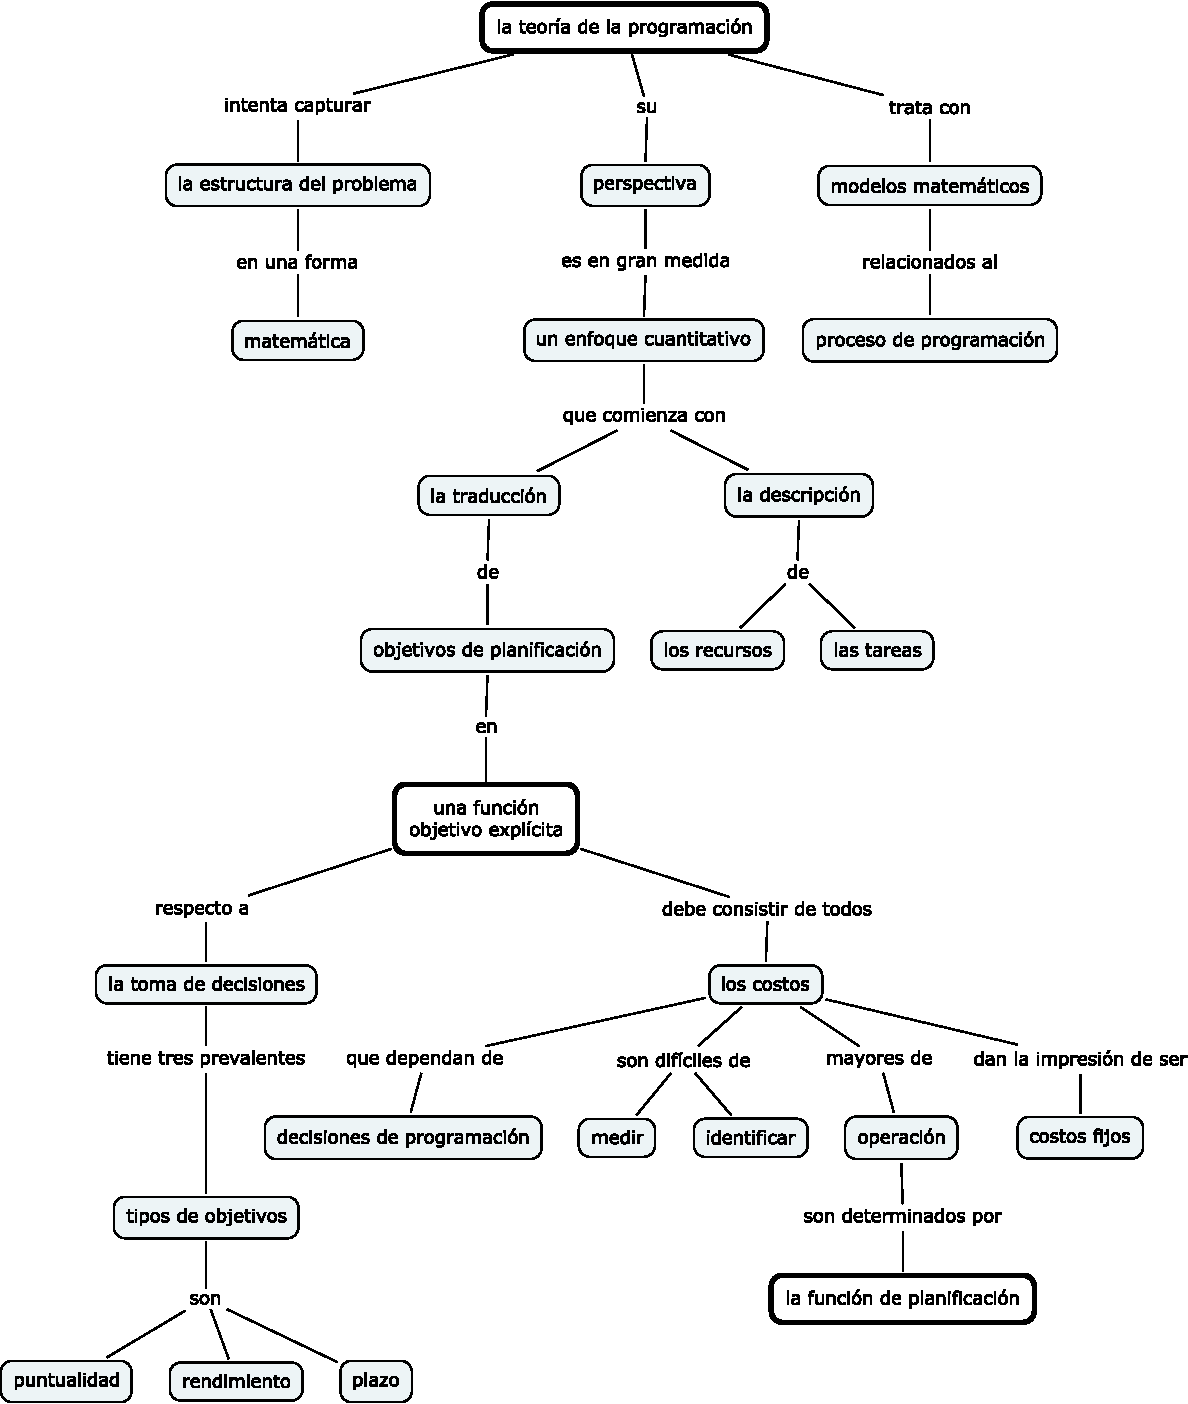
\includegraphics[height=.90\textheight]{media/marco_programacion.pdf}
\caption[El marco de la programación]{El marco de la programación}
\label{fig:marco_programacion}
\end{figure}

\subsection{Función administrativa de planificación y criterios de evaluación}

Según \citet[p.~1]{TKindt2002}, la teoría de la programación aparece a mediados de la década de los cincuenta. Desde entonces los problemas planteados se han aproximado cada vez más a aplicaciones industriales incrementando por tanto su complejidad. La disposición de los talleres tomados en consideración se asemejan cada vez más y más a lo encontrado en la práctica; al mismo tiempo las restricciones impuestas son cada vez más concretas.  Paradójicamente, la literatura muestra que en la mayoría de los problemas planteados, los programas son evaluados por un \textbf{único} criterio.

Durante las diferentes etapas de planificación distintos criterios pueden ser considerados. A un nivel estratégico, una \textbf{planificación de largo alcance} puede contemplar varios años, los objetivos se preocupan con la minimización de costos relacionados a los planes de inversión para materiales, finanzas, o personal, relacionados a la elección de nuevas oportunidades de negocio, o al lanzamiento de campañas de publicidad. Para la planificación estratégica en una \textbf{fase de mediano plazo} con varios meses en mente, los objetivos se enfocan a la minimización de costos: costos de inventario, costos de transporte de insumos, costos de modificación en la capacidad de producción, costos de lanzamiento, costos de modificación de sistemas de producción entre otros. Durante una fase de planificación o una fase de \textbf{programación a corto plazo} –un periodo de tiempo de una semana– multiples objetivos requieren la atención del ejecutivo de producción: ante todo, debe considerar los retrasos para la satisfacción del cliente, acto seguido, debe minimizar el costo del trabajo en proceso de la producción, y finalmente debe minimizar los costos de producción relacionados al tiempo utilizado para la configuración de la maquinaria o los tiempos muertos de las mismas. Es por ello, que un problema de programación puede contemplar multiples criterios de manera tal que permita ofrecer al dueño del problema soluciones más realistas \citep[p.~1]{TKindt2002}. En la figura \ref{fig:criterios_evaluacion} se ilustran los conceptos anteriores.

\begin{figure}[hbtp]
\centering
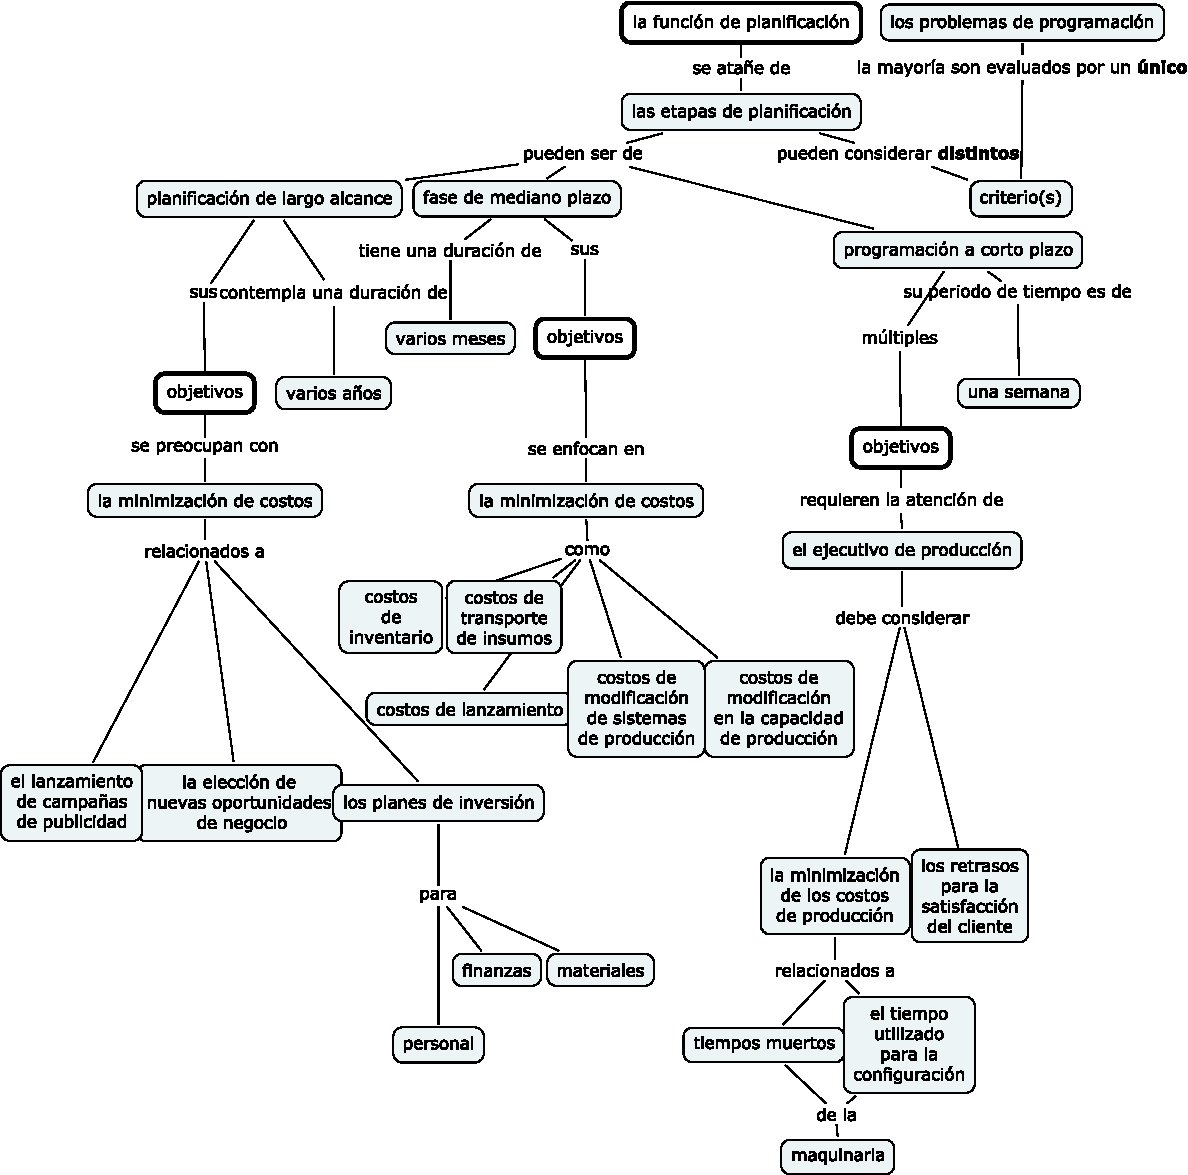
\includegraphics[height=.90\textheight]{media/criterios_evaluacion.pdf}
\caption[Criterios de evaluación]{Criterios de evaluación durante las distintas etapas de planificación}
\label{fig:criterios_evaluacion}
\end{figure}

\section{Tipología de problemas}

\citet[p.~14]{TKindt2002} menciona que en el tema de los problemas de programación se hace una distinción entre su tipología y su notación. Una tipología es una clasificación de los problemas de acuerdo a su naturaleza. En la programación usualmente está basada en el contexto de las máquinas y en las particularidades de los trabajos. Una notación nos permite referirnos rápidamente a un problema, siendo así que es posible construir una base de datos del conjunto de problemas vistos en la literatura.

Existen diferentes tipologías de problemas de programación en la literatura. En la figura \ref{fig:typology_maccarthy} se presenta una generalización del trabajo hecho por \citet{maccarthy1993addressing} (como está citado en \citealp[p.~14]{TKindt2002}). En los problemas de programación el objetivo es determinar una secuencia para cada máquina y un tiempo de inicio para cada operación. En problemas de programación y asignación con etapas se pueden definir, independientemente de cada operación, etapas de máquinas. Una máquina pertenece a una sola etapa. Entonces, se combina cada operación con una etapa, y una operación puede ser procesada por cualquier máquina de su etapa. Por lo tanto, se incorpora un problema de asignación al problema inicial de programación. Ya no es suficiente determinar el tiempo de inicio para las operaciones, sino es necesario también establecer la asignación de las operaciones en las máquinas. Lo mismo ocurre para los problemas generales de programación y asignación en donde un conjunto de máquinas es pormenorizado para cada operación. Por supuesto, una máquina puede existir en más de un conjunto y una operación puede ser llevada a cabo por cualquier máquina perteneciente al mismo conjunto \citep[p.~14,~15]{TKindt2002}.

\begin{figure}[hbtp]
\centering
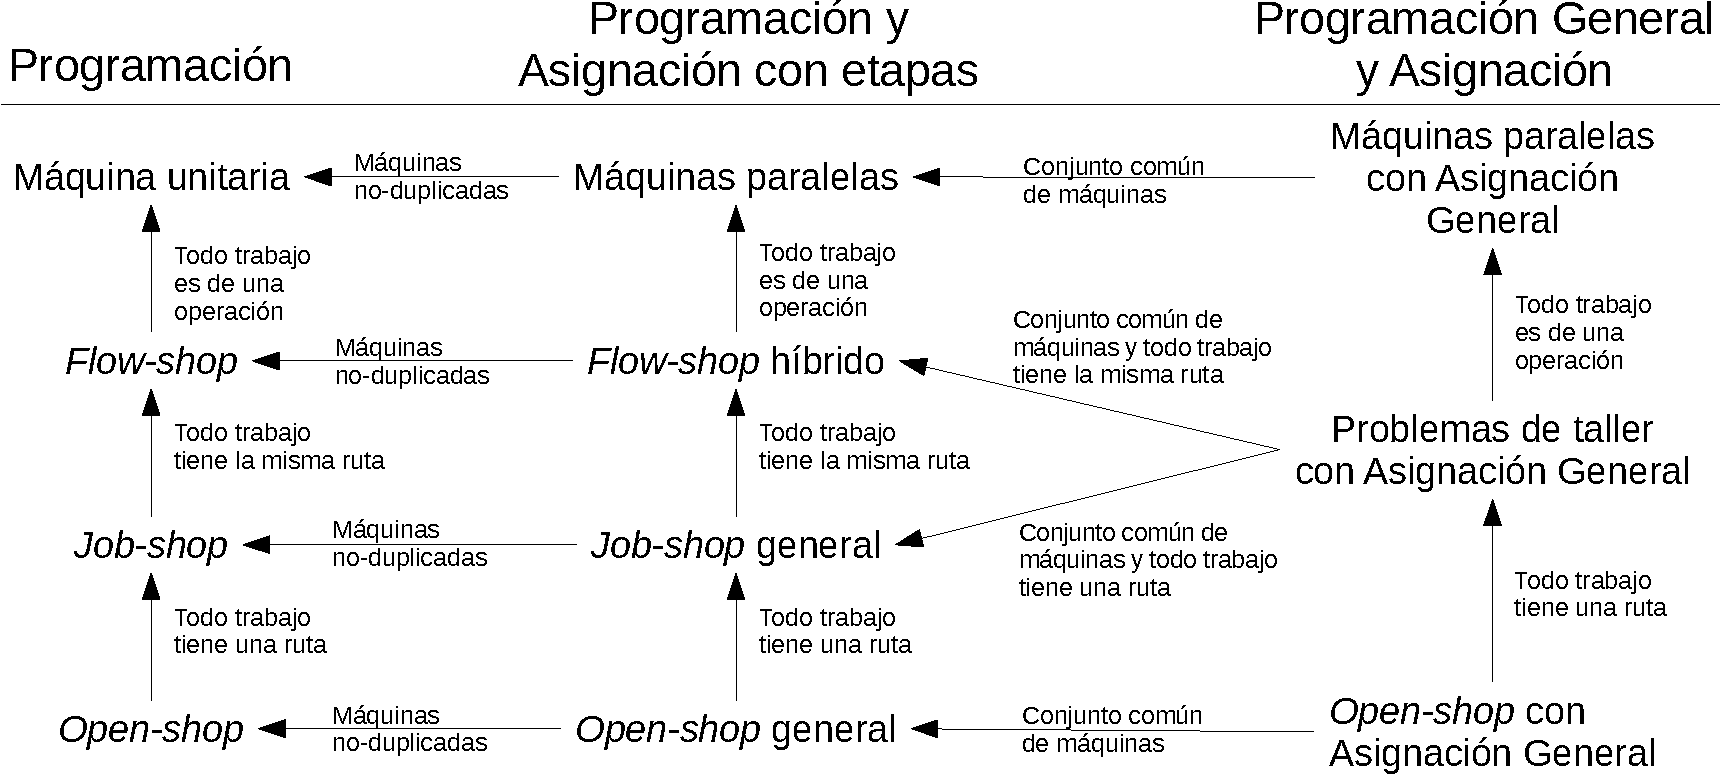
\includegraphics[width=.9\textwidth]{media/typology_maccarthy_spanish.pdf}
\caption[Tipología basada en el contexto de máquinas y operaciones]{Tipología generalizada de problemas de programación de acuerdo a las proposiciones de \citet{maccarthy1993addressing}. De \textit{Multicriteria Scheduling: Theory, Models and Algorithms}, por V. \citeauthor{TKindt2002}, \citeyear{TKindt2002}, p.~15. Derechos reservados [2006] por \textit{Springer-Verlag Berlin Heidelberg}.}
\label{fig:typology_maccarthy}
\end{figure}

La tipología anterior hace uso del entorno de las máquinas y las operaciones para distinguir los problemas. Existen otras tipologías, se pueden estudiar los problemas de acuerdo sus distintas características –véase la fig \ref{fig:typology_cubic}–:

\begin{enumerate}[1]
\item \textbf{determinístico vs. estocástico}. En la situación donde todas las características del problema son bien conocidos, se habla de un problema \textbf{determinístico}. Por otra parte, algunas características pueden consistir de variables aleatorias de ley de probabilidad conocida. En este caso se habla de un problema \textbf{estocástico}.
\item \textbf{unitario vs. repetitivo}. Si las operaciones aparentan ser cíclicas, se trata de un problema \textbf{repetitivo}. En cambio, si cada operación corresponde a un producto único se dice que el problema es \textbf{unitario}.
\item \textbf{estático vs. dinámico}. Si toda la información del problema es conocida al mismo tiempo es un problema \textbf{estático}. Para algunos problemas, un programa puede haber sido elaborado con cierta información y ser ejecutado mientras aparecen nuevas operaciones en el sistema. Entonces el programa anterior tiene que ser restablecido «al momento». Estos problemas se les conoce como \textbf{dinámicos}.
\end{enumerate}

\begin{figure}[hbtp]
\centering
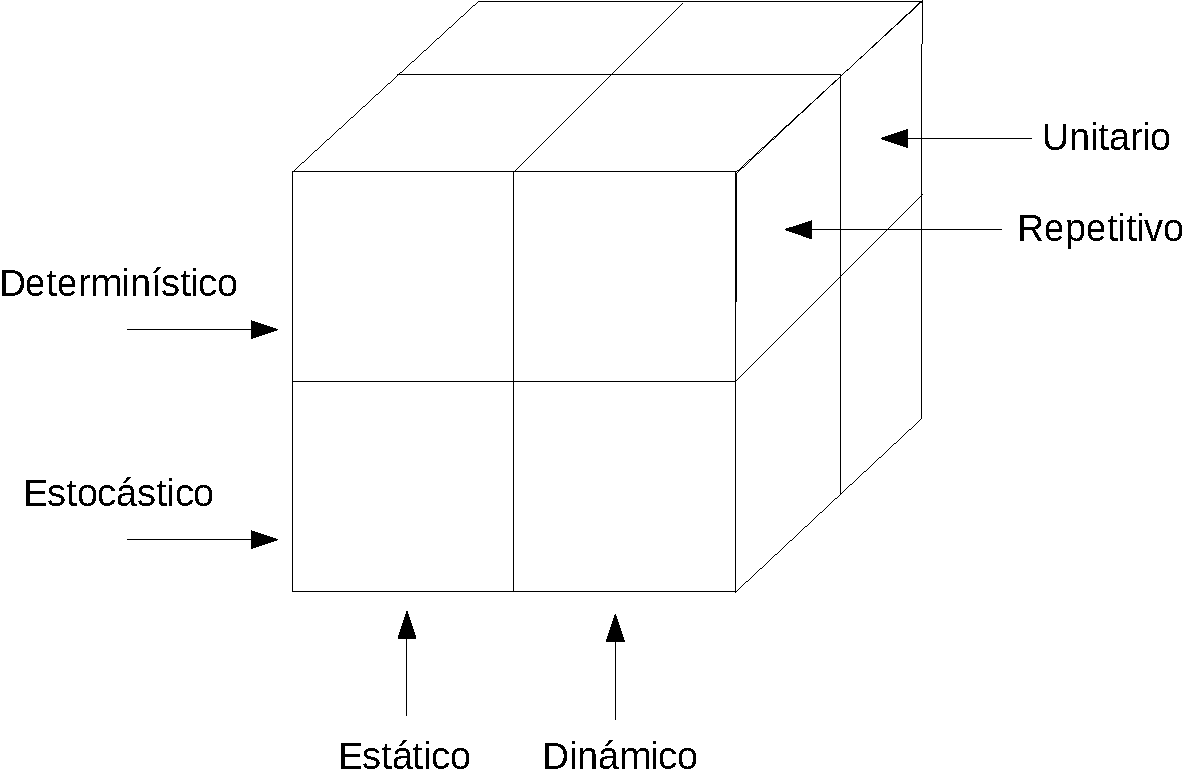
\includegraphics[width=.8\textwidth]{media/typology_cubic.pdf}
\caption[Tipología basada en características]{Tipología de los problemas de programación de acuerdo a sus características. De \textit{Multicriteria Scheduling: Theory, Models and Algorithms}, por V. \citeauthor{TKindt2002}, \citeyear{TKindt2002}, p.~16. Derechos reservados [2006] por \textit{Springer-Verlag Berlin Heidelberg}.}
\label{fig:typology_cubic}
\end{figure}

Estas dos tipologías son complementarias pues es posible trabajar, como ejemplo, con un problema \textit{flow-shop} determinístico, sea unitario o estático. Como será evidente en la próxima sección, la notación tradicional de los problemas de programación es un reflejo de estas tipologías \citep[p.~16]{TKindt2002}.

\section{Notación}

De acuerdo a \citet[p.~13]{Pinedo1995}, en todos los problemas de programación se considera que el número de trabajos y el número de máquinas son finitos. El número de trabajos es denominado por $n$ y el número de máquinas por $m$, la máquina número $k$ se representa por $M_k$. Se denota con $J_i$ al trabajo número $i$, con $n_i$ al número de operaciones del trabajo $J_i$, con $O_{i,j}$ a la operación $j$ del trabajo $J_i$ \citep[p.~7-8, p.~13]{TKindt2002,Pinedo1995}.
Una síntesis completa de la notación es proporcionada en el apéndice A. Los siguientes atributos están asociados a un trabajo $j$.

\textbf{Tiempo de procesamiento} ($p_{i,j}$) La $p_{i,j}$ representa el tiempo de procesamiento de un trabajo $j$ en una máquina $i$. El subíndice $i$ es omitido si el tiempo de procesamiento del trabajo $j$ no depende de la máquina o si el trabajo $j$ va a ser procesado únicamente en una máquina dada \citep[p.~14]{Pinedo1995}.

\textbf{Fecha de liberación} ($r_j$) La fecha de liberación $r_j$ de un trabajo $j$ también es conocida como fecha de disponibilidad. Es cuando el trabajo llega al sistema, en otras palabras, es el tiempo más próximo de inicio en el que el trabajo $j$ puede empezar su procesamiento \citetext{p.~14}.

\textbf{Fecha de cierre} ($d_j$) La fecha de cierre $d_j$ del trabajo $j$ representa la fecha comprometida de compleción o envío. La compleción de un trabajo después de su fecha de cierre \textit{es} permitida, pero se incurre en una penalización. Cuando una fecha de cierre \textit{debe} ser cumplida se le llama \textit{fecha límite} y es denotada por $\bar{d}_j$ \citetext{p.~14}.

\textbf{Peso} ($w_j$) El peso $w_j$ del trabajo $j$ es básicamente un factor de prioridad, denotando la importancia del trabajo $j$ en relación a otros trabajos en el sistema. Por ejemplo, este peso puede representar el costo actual de mantener el trabajo en el sistema. Este costo podría ser un activo o un costo de inventario; también podría representar la cantidad de valor ya agregado al trabajo \citetext{p.~14}.

\begin{table}
\centering
\begin{tabular}{c p{12cm}}
\toprule
\multicolumn{1}{c}{Notación} & \multicolumn{1}{c}{Significado} \\
  \midrule
  $n$                         & Número de trabajos.                                                                                                                                                  \\
  $m$                         & Número de máquinas.                                                                                                                                                  \\
  $J_i$                       & Trabajo número $i$, $i=1,\dots,n$.                                                                                                                                   \\
  $n_i$                       & Número de operaciones del trabajo $J_i$, seguido tenemos que $n_i=m, \forall i, i=1,\dots,n$.                                                                        \\
  $M_j$                       & Máquina número $j$, $j=1,\dots,m$                                                                                                                                    \\
  $O_{i,j}$                   & Operación $j$ del trabajo $J_i$                                                                                                                                      \\
  $r_i (r_{i,j})$             & Tiempo de liberación del trabajo $J_i$ (Respectivamente para la operación $O_{i,j}$).                                                                                \\
  $p_{i,j}$                   & Tiempo de procesamiento de la operación $O_{i,j}$. Cuando existe una única operación por trabajo se usa la notación $p_i$.                                           \\
  $d_i (d_{i,j})$             & Fecha de cierre del trabajo $J_i$ (Respectivamente para la operación $O_{i,j}$).                                                                                     \\
  $\bar{d}_i (\bar{d}_{i,j})$ & Fecha límite del trabajo $J_i$ (Respectivamente para la operación $O_{i,j}$). El trabajo $J_i$ (resp. para $O_{i,j}$) no puede ser completado después de esta fecha. \\
  $w_i (w_{i,j})$             & Peso asociado al trabajo $J_i$ (Respectivamente para la operación $O_{i,j}$).                                                                                        \\
  \bottomrule
\end{tabular}
\caption{Datos generales de un problema de programación}
  \label{tab:problem_data}
\end{table}

Al hacer frente a un problema de programación, se le debe identificar antes de buscar su solución. Aceptando que el problema es complicado y para saber si ya ha sido resuelto en la literatura, se hace uso de una notación reconocida. Con este propósito se han creado «modelos» de talleres, los cuales difieren uno de otro por su composición y la organización de sus recursos \citep[p.~7]{TKindt2002}. Un problema de programación es descrito por una tripleta $\alpha\: \lvert \: \beta\: \lvert \: \gamma$. El campo $\alpha$ describe el entorno de la máquina y contiene únicamente un registro. El campo $\beta$ provee detalles de las características del procesamiento y restricciones, puede no tener registro alguno, un solo registro o múltiples registros. El campo $\gamma$ describe el objetivo a ser minimizado y frecuentemente contiene un solo registro \citep[p.~14]{Pinedo1995}.

\subsection{Campo $\alpha$ - entornos}

Los posibles entornos de máquinas especificadas en el campo $\alpha$ se presentan a continuación agrupados de acuerdo al tipo de problema de programación que se busca resolver.

\subsubsection{Problemas de programación sin asignación}

En este tipo de problemas se busca encontrar un tiempo de inicio de procesamiento para cada operación. Distintos tipos de configuraciones son comúnmente encontrados \citep[p.~8]{TKindt2002}:

\textbf{Máquina singular} ($1$) El caso de una máquina singular es el más simple de todos los entornos de máquina posibles y es un caso especial de todos los demás entornos de máquina más complicados. Concierne a un taller de trabajo básico o uno en donde una máquina singular presenta un problema de programación real. Una área de aplicación directa se encuentra en la computación, si pensamos en la máquina singular como el procesador singular de un ordenador; los trabajos a ser procesados son necesariamente mono-operación \citep[p.~8, p.~14]{TKindt2002,Pinedo1995}.

\textbf{Flowshop} ($Fm$) Existen $m$ máquinas disponibles en el taller de trabajo. Cada trabajo tiene que ser procesado en en cada una de las $m$ máquinas. Todos los trabajos tienen que seguir la misma ruta de procesamiento, estos, al ser completados en una máquina se unen a la cola para la siguiente máquina. Usualmente, todas las colas se presumen operantes bajo la dinámica  «primero en entrar, primero en salir» (\textit{First In First Out; FIFO}), de manera tal, que un trabajo no puede adelantarse a otro mientras espera en la cola \citep[p.~8, p.~15]{TKindt2002,Pinedo1995}.

\textbf{Job-shop} ($Jm$) En un taller de trabajo con $m$ máquinas cada trabajo tiene su propia ruta de procesamiento a seguir, esto es, el trabajo utiliza los recursos en un orden propio \citep[p.~8, p.~15]{TKindt2002,Pinedo1995}.

\textbf{Open-shop} ($Om$) Existen $m$ máquinas. Cada trabajo debe ser procesado en cada una de las máquinas $m$. Sin embargo, algunos de estos tiempos de procesamiento pueden ser instantáneos. No hay restricciones respecto a la construcción de la ruta de procesamiento que cada trabajo debe de seguir en el entorno de máquinas. La herramienta de programación está facultada para determinar la ruta de cada trabajo y distintos trabajos pueden tener distintas rutas, por lo tanto estos pueden usar las máquinas en cualquier orden \citep[p.~8, p.~15]{TKindt2002,Pinedo1995}.

\textbf{Mixed shop} ($X$) Este entorno es una combinación de los anteriores, en donde existen múltiples máquinas disponibles en el taller y algunos de los trabajos pueden compartir la misma ruta de procesamiento \citep[p.~8]{TKindt2002}.

\subsubsection{Problemas de programación y asignación con etapas}

Las máquinas están agrupadas en etapas bien definidas y cada máquina pertenece a una etapa únicamente. En todos los casos, las máquinas de una etapa son capaces de desempeñar las mismas operaciones. Para llevar a término una operación es necesario elegir alguna de las máquinas disponibles, de manera tal, que el problema es dual: se persigue la asignación de una máquina para cada operación y la secuenciación de las operaciones en las máquinas.

En cada etapa se puede presentar los siguientes tipos de configuraciones \citep[p.~8]{TKindt2002}:

\textbf{Máquinas idénticas en paralelo} ($Pm$) Hay una cantidad idéntica de máquinas en paralelo. El trabajo $j$ requiere una operación única y puede ser procesado por cualquiera de las máquinas $m$ o por cualquiera que pertenezca a un subconjunto dado, todas las operaciones tienen el mismo tiempo de procesamiento en todas las máquinas. Si el trabajo $j$ no puede ser procesado en cualquier máquina, sino únicamente en alguna perteneciente a un subconjunto $M_j$, entonces la entrada $M_j$ aparece en el campo $\beta$ \citep[p.~14, p.~8]{Pinedo1995,TKindt2002}.

\textbf{Máquinas en paralelo con velocidades distintas} ($Qm$) Hay múltiples máquinas $m$ en paralelo con distintas velocidades.
El tiempo de procesamiento de una operación $O_{i,j}$ en la máquina $M_k$ es igual a $p_{i,j,k} = q_{i,j}/v_k$ en donde $q_{i,j}$ puede ser el número de componentes que deben ser procesados en la operación $O_{i,j}$, y $v_k$ es el número de componentes que la máquina $M_k$ puede procesar por unidad de tiempo.

Cuando todo el procesamiento del trabajo $j$ es llevado a cabo en la misma máquina $k$, el tiempo $p_{i,j,k}$ que las operaciones $i$ del trabajo $j$ utilizan de la máquina $k$ es igual a $p_{i,j}/v_k$. Este entorno es referido como máquinas uniformes. Si todas las máquinas tienen la misma velocidad, esto es $v_k = 1$ para toda $jk$ y $p_{i,j,k} = p_{i,j}$, entonces el entorno es idéntico al anterior \citep[p.~14, p.~8]{Pinedo1995,TKindt2002}.

\textbf{Máquinas no-relacionadas en paralelo} ($Rm$) Este entorno es una generación más extensa del entorno anterior. El tiempo de procesamiento de la operación $O_{i,j}$ en la máquina $M_k$ es igual a $p_{i,j,k}$ y es un dato del problema. Por supuesto, así como la asignación de la operación $O_{i,j}$ es desconocida, también lo es su tiempo de procesamiento \citep[p.~14, p.~9]{Pinedo1995,TKindt2002}.

Universalmente, los problemas de programación y asignación «tradicionales» corresponden a las siguientes configuraciones:
\begin{itemize} 
\item\textbf{Máquinas paralelas} ($P/Q/R$) Existe una sola etapa y los trabajos son mono-operación.
\item\textbf{Flowshop híbrido} ($HF$) Todos los trabajos tienen la misma ruta de producción, y por lo tanto hacen uso de las etapas en el mismo orden.
\item\textbf{Job-shop general} ($GJ$) Cada trabajo tiene una ruta propia.
\item\textbf{Open-shop general} ($GO$) Los trabajos no tienen una ruta fija.
\end{itemize}
Es muy sencillo generalizar estos problemas al suponer que cada operación puede hacer uso de un subconjunto de los recursos de la etapa correspondiente \citep[p.~9]{TKindt2002}.

\subsubsection{Problemas generales de programación y asignación}

Este es el caso más general en donde se supone que cada operación tiene su propio conjunto de máquinas en las cuales pueden ser procesadas. No existe asunción acerca de este conjunto de recursos. Se pueden diferenciar distintos casos \citep[p.~9]{TKindt2002}:

\begin{itemize}
\item Los trabajos son mono-operación, y están confrontados por un problema de \textbf{máquinas paralelas con asignación general}. Estos problemas aparecen en la literatura bajo el nombre de «Problemas de Programación de Máquinas Multi Propósito» (\textit{Multi Purpose Machine Scheduling Problems}) (\textit{P/Q/R MPM SP}) \citep[p.~9]{TKindt2002}.

\item Los trabajos siguen un orden de procesamiento. Es difícil en este caso hace una distinción entre \textit{flowshop} y \textit{job-shop} puesto que los grupos de máquinas utilizados por estos trabajos no son comparables. A esto se le conoce como \textbf{talleres con problemas generales de asignación} (\textit{shops with general assignment problems}) (\textit{"General Shop MPM SP"})

\item Los trabajos no siguen una ruta de procesamiento fija. Este es el caso de los \textbf{talleres-abiertos con problemas generales de asignación} («\textit{Open-shop MPM SP}»)

\end{itemize}

\begin{table}
\centering
\begin{tabular}{l p{12cm}}
\toprule
  \multicolumn{1}{c}{Valor} & \multicolumn{1}{c}{Significado} \\
  \midrule
  $0$ & Máquina singular \\
  $P,Q,R$ & Máquinas paralelas idénticas, proporcionales o ajenas \\
  $F,J,O,X$ & Flowshop, job-shop, open-shop, mixed-shop. \\
  $HF$ & Flowshop híbrido \\
  $GO$ & Open-shop general \\
  $GJ$ & Job-shop general \\
  $\{P,Q,R\}MPM$ & Máquinas paralelas (del tipo P, Q o R) con un problema general de asignación \\
  $G M P M$ & Shop con un problema general de asignación \\
  $O M P M$ & Open-shop con un problema general de asignación \\
  \bottomrule
\end{tabular}
  \caption{El campo $\alpha$}
  \label{tab:notation_alpha}
\end{table}

\subsection{Campo $\beta$ - restricciones}

Una solución de un problema de programación debe siempre satisfacer un cierto número de restricciones, ya sean explícitas o implícitas. En un problema \textit{flowshop} está implícito que los trabajos deben ser procesados de acuerdo a una ruta definida y por consiguiente, una operación no puede comenzar mientras su precedente permanezca incompleta. 
Por otra parte, la ocurrencia de los distintas fechas de liberación constituye una restricción que debe ser establecida precisamente. En esta sección se describen las restricciones explícitas más comúnmente encontradas en la programación. Un resumen más completo se presenta en el apéndice A \citep[p.~9-10]{TKindt2002}. 

Hay distintos tipos de restricciones relacionadas a las \textbf{fechas de cierre}. Están las fechas de cierre que no deseamos rebasar, aun cuando se tolera su compleción después de tiempo. Ellas corresponden a un acuerdo comprometido que es negociable. Están aquellas fechas de cierre que son imperativas, también llamadas fechas límite, y que no pueden ser rebasadas. Típicamente, corresponden a una fecha de inauguración donde el fabricamente debe presentar su producto, o incluso puede ser la fecha de salida de un camión de carga. Estas fechas no puede ser rebasadas, por consiguiente ningún retraso puede ser permitido. Los problemas en dónde se encuentran estas restricciones generalmente son problemas de toma de decisión: estás fechas pueden o no pueden ser logradas. Cuando es posible alcanzarlas, se está satisfecho con la solución factible o adicionalmente se busca intentar minimizar algún otro criterio \citep[p.~10]{TKindt2002}.

Las restricciones relacionadas a los \textbf{tiempos de inicio} son igualmente variadas. Por supuesto, está la fecha de liberación del producto. En ocasiones corresponde con la fecha de la orden. Igualmente, se puede encontrar una fecha de liberación asociada con una operación específica de un trabajo. Esta fecha puede corresponder a la llegada de suministros para la operación. Finalmente, puede suceder que el tiempo de inicio de una operación en particular sea impuesto. En este caso, es cuestión de reunirse con el cliente para que atestigüe la implementación de la operación que él considera crítica en el proceso de manufactura. Estas dos últimas definiciones corresponden a problemas raramente encontrados en la literatura \citep[p.~10]{TKindt2002}.

Algunas de las restricciones comúnmente encontradas en la literatura son las siguientes:

\begin{itemize}
  \item \textbf{Fechas de liberación} ($r_j$) Si este símbolo aparece en el campo $\beta$, entonces el trabajo $j$ no puede comenzar su procesamiento antes de su fecha de liberación $r_j$. Si $r_j$ no aparece en el campo $\beta$, el procesamiento del trabajo $j$ puede comenzar en cualquier momento. En comparación con las fechas de liberación, las fechas de cierre no se especifican en este campo. El tipo de función objetivo da suficiente indicación respecto a si hay o no fechas de cierre \citep[p.~16]{Pinedo1995}.
  \item \textbf{Apropiaciones} ($prmp$) Las apropiaciones implican que no es necesario mantener un trabajo en una máquina, una vez que ha comenzado, hasta su compleción. Es decir, es posible prever la interrupción de una operación de manera que sea posible hacer uso de la máquina para la compleción de algún otro trabajo. La cantidad de procesamiento alcanzado al momento de la interrupción no se pierde al poner de vuelta al trabajo –o al transferirlo a otra máquina en caso de tratarse de máquinas paralelas–, únicamente hace uso de la máquina por el tiempo faltante de su compleción \citep[p.~16, p.~10]{Pinedo1995,TKindt2002}.
  \item \textbf{División} ($split$) Indica que la división está permitida, haciendo posible que una operación se descomponga en múltiples porciones, las cuales pueden ser ejecutadas en una o más máquinas, posiblemente de manera concurrente \citep[p.~10]{TKindt2002}.
  \item \textbf{Restricciones de precedencia} ($prec$) Las restricciones de precedencia pueden aparecer en un entorno de máquina singular o de máquinas paralelas, requiriendo que uno o más trabajos sean completados antes de que otro trabajo pueda comenzar su procesamiento \citep[p.~16]{Pinedo1995}.
  \item \textbf{Procesamiento por lotes} ($batch$) Una máquina puede ser capaz de procesar una cantidad de trabajos de manera simultánea, es decir, puede procesar un lote de trabajos al mismo tiempo. Los tiempos de procesamiento de los trabajos en el lote pueden ser de duración variada y el lote alcanza su compleción hasta que el último trabajo del lote ha sido completado, teniendo como entendido que el tiempo de compleción del lote de trabajos está determinado por el trabajo con el tiempo de procesamiento más prologando \citep[p.~16]{Pinedo1995}.
  \item \textbf{Sin-detenimientos} ($no-wait$) Indica que las operaciones que constituyen a cada trabajo siguen unas a otras sin alguna espera \citep[p.~11]{TKindt2002}.
  \item \textbf{Permutación} ($prmu$) Una restricción que puede aparecer en los entornos \textit{flowshow} es que las filas delante de cada máquina operan de acuerdo a las normas «primero en entrar, primero en salir» (\textit{First In First Out; FIFO}). Esto implica que el órden (permutación) en que los trabajos atraviesan la primera máquina se mantienen durante todo el sistema \citep[p.~17]{Pinedo1995}.
\end{itemize}

\begin{table}
\centering
\begin{tabular}{l p{12cm}}
\toprule
  \multicolumn{1}{c}{Valor} & \multicolumn{1}{c}{Significado} \\
  \midrule
  $prec$ & Hay restricciones generales de precedencia entre las operaciones. \\
  $chains$ & Existen restricciones de precedencia que conforman un conjunto de cadenas entre operaciones. \\
  $split$ & La división de una operación en partes está permitida y éstas pueden ser procesadas simultáneamente. \\
  $pmtn$ & Las operaciones pueden ser interrumpidas y retomadas más tarde en cualquier otra máquina \\
  $no-wait$ & Para cada trabajo, cuando una operación es completada la siguiente debe comenzar. \\
  \bottomrule
\end{tabular}
\caption{El campo $\beta$}
\label{tab:notation_beta}
\end{table}

\subsection{Campo $\gamma$ - criterio de optimalidad}

De acuerdo a \citet[p.~12]{TKindt2002}, con el fin de evaluar un programa se puede hacer uso de un cierto número de criterios. Ocasionalmente se puede querer que un criterio se acerque lo más posible a un valor de referencia dado. Aquí se está en la frontera entre las nociones de criterios y restricciones. Si una restricción representa un hecho que en definitiva debe de ser respetado, la optimación de un criterio permite más bien cierto grado de libertad. Como ejemplo, la declaración de que ningún trabajo debe completarse tarde de acuerdo a su fecha de cierre no deja margen alguno en la construcción del programa; incluso puede ser que no exista un programa factible en tal situación. Por otra parte, la minimización del número de trabajos tardíos permite garantizar que siempre habrá una solución, aun cuando para lograr esto ciertos trabajos puedan ser tardíos. Desde un punto de vista práctico, la diferencia entre un criterio y una restricción es únicamente aparente para quien está facultado en la toma de decisiones.

\citet[p.~12,~13]{TKindt2002} prosiguen explicando que ciertos criterios son equivalentes y es por eso que se presentan conjuntamente: la minimización de uno u otro conlleva a la misma solución óptima aun si el valor del criterio no es el mismo en ambos casos. Algunos problemas de programación carecen de criterios a ser minimizados. En este caso se trata de un problema de factibilidad, también llamado un problema de decisión: ¿existe una solución que satisfaga las restricciones existentes?

Los criterios se pueden clasificar en dos grandes familias: los criterios «minimax», los cuales representan el valor máximo de un conjunto de funciones a ser minimizadas, y los criterios «minisum», quienes representan una suma de funciones a ser minimizadas \citep[p.~13]{TKindt2002}.

\begin{table}
\centering
\begin{tabular}{l l p{8cm}}
\toprule
\multicolumn{1}{l}{Criterio} & \multicolumn{1}{l}{Expresión} & \multicolumn{1}{l}{Significado} \\
  \midrule
  $C_{\max}$            & $\underset{i=1,\dots,n}{\max} (C_i)$                                             & Makespan, o tiempo máximo de compleción.                                                                                          \\[12pt]
  $T_{\max}$            & $\underset{i=1,\dots,n}{\max} (\max (C_i-d_i;0))$                                & Tardanza máxima de los trabajos                                                                                                   \\[12pt]
  $L_{\max}$            & $\underset{i=1,\dots,n}{\max} (C_i-d_i)$                                         & Retardo máximo de los trabajos                                                                                                    \\[12pt]
  $E_{\max}$            & $\underset{i=1,\dots,n}{\max} (\max(d_i-C_i;0))$                                 & Precocidad máxima de los trabajos                                                                                                 \\[12pt]
  $\fint_{\max}$        & $\underset{i=1,\dots,n}{\max} (\fint_i)$                                         & Función genérica de costo máximo. Generalmente, se asume como una función creciente de los tiempos de compleción de los trabajos. \\
  $\bar{C} (\bar{C}^w)$ & $\overset{n}{\underset{i=1}{\sum}}C_i (\overset{n}{\underset{i=1}{\sum}}w_iC_i)$ & Tiempos (ponderados) promedio de compleción de los trabajos.                                                                      \\
  $\bar{T} (\bar{T}^w)$ & $\overset{n}{\underset{i=1}{\sum}}T_i (\overset{n}{\underset{i=1}{\sum}}w_iT_i)$ & Tardanza (ponderada) promedio de los trabajos.                                                                                    \\
  $\bar{U} (\bar{C}^w)$ & $\overset{n}{\underset{i=1}{\sum}}U_i (\overset{n}{\underset{i=1}{\sum}}w_iU_i)$ & Cuantía (ponderada) de trabajos con retraso.                                                                                      \\[12pt]
  $\bar{E} (\bar{T}^w)$ & $\overset{n}{\underset{i=1}{\sum}}E_i (\overset{n}{\underset{i=1}{\sum}}w_iE_i)$ & Precocidad (ponderada) promedio de los trabajos.                                                                                  \\
  — & & Sin criterio; es un problema de factibilidad.    \\
  \bottomrule
\end{tabular}
\caption{El campo $\gamma$}
\label{tab:notation_gamma}
\end{table}

\subsubsection[Criterio «minimax»]{Minimización de una función máxima: criterio «minimax»}

\citet[p.~18]{Pinedo1995} explica que el objetivo a minimizar casi siempre es una función de los tiempos de compleción de los trabajos, los cuales, por supuesto, dependen del programa. 
El tiempo de compleción de la operación del trabajo $j$ en la máquina $i$ se denota por $C_{i,j}$. El tiempo de salida del sistema del trabajo $j$ –su tiempo de compleción en la última máquina que utilizó para su procesamiento– se denota con $C_j$.
%
El retardo (\textit{lateness}) de un trabajo $j$ se define como 
\[ L_j = C_j - d_j, \]
el cual es positivo cuando el trabajo $j$ es completado tardíamente y negativo cuando es completado precozmente. La tardanza (\textit{tardiness}) de un trabajo $j$ se define como
\[ T_j = \max(C_j - d_j, 0) = \max(L_j, 0). \]
La diferencia entre tardanza y retardo se fundamenta en el hecho de que la tardanza nunca es negativa. La unidad de penalización (\textit{unit penalty}) de un trabajo $j$ se define como
\[ U_j = \left\{
    \begin{array}{ll}
      1 & \mbox{si } C_j > d_j \\
      0 & \mbox{en caso contrario}
    \end{array}
  \right. \]
El retardo, la tardanza y la unidad de penalización son las tres funciones relacionadas a la penalización de las fechas de cierre, básicas en la literatura. La forma que toman estas funciones está mostrada en la figura \ref{fig:penalty_fun}.

\begin{figure}[hbtp]
\centering
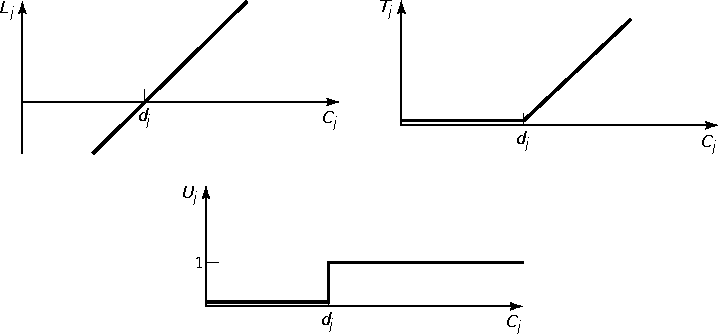
\includegraphics[width=.8\textwidth]{media/penalty_functions.pdf}
\caption[Funciones de penalización]{Funciones de penalización relacionadas a las fechas de cierre. De \textit{Scheduling: Theory, Algorithms, and Systems}, por M. \citeauthor{Pinedo1995}, \citeyear{Pinedo1995}, p.~18. Derechos reservados [2008] por \textit{Springer Science+Business Media, LLC}.}
\label{fig:penalty_fun}
\end{figure}

Algunos posibles ejemplos de funciones objetivo a ser minimizadas son:

\textbf{Makespan} ($C_{\max}$) El criterio clásico es, sin lugar a dudas, aquel que mide el tiempo de compleción de todos los trabajos. Este criterio se denota por $C_{max}$ y es conocido como «makespan». Se define a $C_{max} = \underset{i=1,\dots,n}{\max}(C_i)$, siendo $C_i$ el tiempo de compleción del trabajo $J_i$. Para simplificar la notación, se escribe «$\max$» en lugar de «$\underset{i=1,\dots,n}{\max}$» cuando no existe ambigüedad posible. $C_{max}$ es la duración total del programa. Un makespan mínimo usualmente implica una buena utilización de las máquinas \citep[p.~13, p.~18]{TKindt2002,Pinedo1995}.

\textbf{Tiempo ponderado total de compleción} ($\sum w_jC_j$) La suma de los tiempos ponderados de compleción de los $n$ trabajos proporciona una indicación de la participación total o de los costos de inventario incurridos por el programa. La suma de los tiempos de compleción aparece frecuentemente en la literatura con el término «tiempo de flujo» (\textit{flow time}). El tiempo ponderado total de compleción, por ende, es llamado «tiempo de flujo ponderado» (\textit{weighted flow time}) \citep[p.~18]{Pinedo1995}.

\textbf{Cuantía ponderada de trabajos tardíos} ($\sum w_jU_j$) 
La cuantía ponderada de trabajos tardíos no es únicamente una métrica de interés académico, reiteradamente es un objetivo en la práctica y es una medida que se puede asentar fácilmente \citep[p.~19]{Pinedo1995}.

Existen otros criterios basados únicamente en el tiempo de compleción de los trabajos, como:

\begin{itemize}
\item$F_{\max} = \max(F_i)$ siendo $F_i = C_i - r_i$: el tiempo máximo utilizado en el taller, o incluso aún, la duración del descanso, con $r_i$ siendo la fecha de liberación del trabajo $J_i$.
\item$I_{\max} = \max(I_k)$: siendo $I_k$ la suma de los tiempos muertos en el recurso $M_k$.
\end{itemize}
%
De igual manera, se encuentran en la literatura criterios que están basados en las fechas de cierre $d_i$, $\forall i = 1,\dots,n$ de los trabajos. Sobresalen los siguientes criterios:
%
\begin{itemize}
  \item $L_{\max} = \max(L_i)$ siendo $L_i = C_i - d_i$: el máximo retardo (\textit{lateness}).
  \item $T_{\max} = \max(T_i)$ siendo $T_i = \max(0; C_i - d_i)$: la máxima tardanza (\textit{tardiness}).
  \item $E_{\max} = \max(E_i)$ siendo $E_i = \max(0; d_i - C_i)$: la máxima precocidad (\textit{earliness}) \citep[p.~13]{TKindt2002}.
\end{itemize}

Generalmente, $\fint_{\max}$ se refiere al criterio ordinario «minimax», el cual es una función no\nobreakdash-decreciente de los tiempos de compleción de los trabajos en $C_1,\dots,C_n$, estas funciones objetivo son llamadas medidas de desempeño regulares. Este no es el caso para el criterio $E_{\max}$ \citep[p.~13]{TKindt2002}. Recientemente los investigadores han empezados a estudiar funciones objetivo que no son regulares. Por ejemplo, cuando el trabajo $j$ tiene la fecha de cierre $d_j$, puede estar sujeto a una penalización por precocidad, en donde la «precocidad» del trabajo $j$ se define como 
\[ E_j = \max (d_j - C_j, 0) \]
Esta penalización por precocidad es no\nobreakdash-decreciente en $C_j$. Un objetivo como la precocidad total más la tardanza total, sería:
\[ \sum_{j=1}^{n}E_{j}+\sum_{j=1}^{n}T_{j} \]
es por lo tanto no\nobreakdash-regular. Un objetivo más general que no es regular es la precocidad ponderada total más la tardanza ponderada total, que es:
\[ \sum_{j=1}^{n}w'_jE_{j}+\sum_{j=1}^{n}w''_jT_{j} \]
El peso asociado a la precocidad del trabajo $j$ ($w'_j$) puede ser diferente al peso asociado a la tardanza del trabajo $j$ ($w''_j$) \citep[p.~19]{Pinedo1995}.

\subsubsection[Criterio «minisum»]{Minimización de una función de suma: criterio «minisum»}

Los criterios «minisum» son usualmente más dificiles de optimar que su contraparte «minimax» \citep[p.~13]{TKindt2002}. Entre los criterios existentes en la literatura están los siguientes:

\begin{itemize}
  \item $\bar{C}$ para designar $\frac{1}{n}\sum C_i$ ó $\sum C_i$. Este criterio representa el tiempo de compleción promedio o el tiempo total de compleción de los trabajos.
  \item $\bar{C}^w$ para designar $\frac{1}{n} \sum w_iC_i$, $\frac{1}{\sum w_i}\sum w_iC_i$ ó $\sum w_iC_i$. Este criterio representa el tiempo ponderado promedio de compleción o el tiempo ponderado total de compleción de los trabajos.
  \item $\bar{F}$ para designar $ \frac{1}{n}\sum F_i $ ó $\sum F_i$. La optimación de este criterio es equivalente a la optimación del criterio $\bar{C}$. Es lo mismo para el criterio $\bar{F}^w$ respecto al criterio $\bar{C}^w$.
  \item $\bar{T}$ para designar $\frac{1}{n}\sum T_i$ ó $\sum T_i$. Este criterio designa la tardanza promedio o la tardanza total de los trabajos.
  \item $\bar{T}^w$ para designar $\frac{1}{n}\sum w_iT_i$, $\frac{1}{\sum w_i}\sum w_iT_i$ ó $\sum w_iT_i$. Este criterio designa la tardanza ponderada promedio o la tardanza ponderada total de los trabajos.
  \item $\bar{U}$ para designar $\sum U_i$ que es la cuantía de los trabajos retrasados con $U_i=1$ si el trabajo $J_i$ está retrasado y $U_i=0$ en caso contrario.
  \item $\bar{U}^w$ para designar $\frac{1}{n}\sum w_iU_i$, $\frac{1}{\sum w_i}\sum w_iU_i$ ó $\sum w_iU_i$ los cuales representan la cuantía ponderada de los trabajos retrasados.
  \item $\bar{E}$ es el promedio de precocidad de los trabajos.
  \item $\bar{E}^w$ es el promedio ponderado de precocidad de los trabajos \citep[p.~14]{TKindt2002}.
\end{itemize}

\citet[p.~14]{TKindt2002} concluye señalando que en general, $\bar{\fint}$ designa un criterio «minisum» ordinario el cual es usualmente una función no\nobreakdash-decreciente de los tiempos de compleción de los trabajos. Este no es el caso para el criterio $\bar{E}$.

\subsection{Ejemplos de la notación}
\label{sub:notacion_ejemplos}

\subsubsection{Un entorno de máquina singular}

\begin{simple}
  $1 \: \lvert \: r_j, prmp \: \lvert \: \sum w_jC_j$ denota un sistema de máquina singular con el trabajo $j$ entrando al sistema en su fecha de liberación $r_j$. Las apropiaciones son permitidas. El objetivo a ser minimizado es la suma ponderada de los tiempos de compleción \citep[p.~20]{Pinedo1995}.
\end{simple}

\subsubsection{Secuencia subordinada a tiempos de configuración}

\begin{simple}
  $1 \: \lvert \: s_{j,k} \: \lvert \: C_{\max}$ denota un sistema de máquina singular con $n$ trabajos sujetos a una secuenciación subordinada a los tiempos de configuración, en donde el objetivo es minimizar el makespan. Es bien sabido que este problema es equivalente al denominado problema del agente viajero (\textit{travelling salesman problem; TSP}) \citep[p.~20]{Pinedo1995}.
\end{simple}

\subsubsection{Un proyecto}

\begin{simple}
  $P \infty \: \lvert \: prec \: \lvert \: C_{\max}$ denota un problema de programación con $n$ trabajos sujeto a restricciones de precedencia y un número ilimitado de máquinas (o recursos) en paralelo. El tiempo total del proyecto en su totalidad debe ser minimizado. Este tipo de problemas es muy común en planeación de proyectos en la industria de la construcción y ha llevado al desarrollo de técnicas como \textit{CPM} y \textit{PERT} \citep[p.~21]{Pinedo1995}.
\end{simple}.

\subsubsection{Un entorno de máquinas paralelas}

\begin{simple}
  $Pm \: \lvert \: r_j,M_j \: \lvert \: \sum w_jT_j$ denota un sistema con $m$ máquinas en paralelo. El trabajo $j$ arriba en la fecha de liberación $r_j$ y tiene que salir para la fecha de cierre $d_j$. El trabajo $j$ puede ser procesado únicamente en una de las máquinas pertenecientes al subconjunto $\mathcal{M}_j$, si el trabajo $j$ no es completado a tiempo, una penalización $w_jT_j$ es adjudicada. El modelo puede ser aplicado para el problema de asignación siguiente \citep[p.~20]{Pinedo1995}:
\end{simple}

Téngase en consideración la terminal de un aeropuerto mayor. Existen docenas de puertas y cientos de aviones llegan y salen cada día. Las puertas no son todas idénticas y tampoco lo son los aviones. Algunas de las puertas están en sitios con amplio espacio en donde los aviones grandes (\textit{widebodies}) puede ser acomodados con facilidad. Otras puertas están en sitios en donde es difícil hacer pasar a los aviones; ciertos aviones incluso pueden requerir ser remolcados a sus puertas \citep[p.~2,~3]{Pinedo1995}.

Los aviones llegan y salen de acuerdo a cierto itinerario. Sin embargo, éste está sujeto a una cierta cantidad de incertidumbre, la cual se puede deber a situaciones climáticas o por ocurrencias imprevistas en otros aeropuertos. Durante el tiempo que un avión ocupa la puerta los pasajeros entrantes tienen que descender del avión, éste tiene que recibir servicio y los pasajeros salientes deben abordar. El tiempo de salida programado puede ser visto como una fecha de cierre y el desempeño de la aerolínea puede ser evaluado correspondientemente. Sin embargo, si se conoce con antelación que un avión no puede aterrizar en el aeropuerto próximo debido a una congestión anticipada a su hora programada de llegada, entonces el avión no despega —esta política es seguida para conservar combustible—. Si un avión no tiene permitido despegar, las politicas operativas usualmente disponen que los pasajeros permanezcan en la terminar en lugar del avión. Si el abordaje es pospuesto, un avión puede permanecer en la puerta por un periodo extendido de tiempo, impidiendo así que otros aviones hagan uso de la puerta \citep[p.~3]{Pinedo1995}.

El programador debe asignar puertas a los aviones de manera tal que la asignación sea físicamente factible mientras se optiman ciertos objetivos. Esto impolica que el programador tienen que asignar aviones a puertas adecuadas que estén disponibles a sus horas de llegada respectivas. Los objetivos incluyen la minimización del trabajo del personal de la aerolinea y la minimización de los retrasos en los aviones \citep[p.~3]{Pinedo1995}.

En este escenario, las puertas son los recursos y el manejo y servicio de los aviones son las tareas. El arribo de un avión a una puerta representa el tiempo de inicio de la tarea y la salida representa su tiempo de compleción \citep[p.~3]{Pinedo1995}.

\subsubsection{Un \textit{flow-shop} flexible}

\begin{simple}
  $FFc \: \lvert \: r_j \: \lvert \: \sum w_jT_j$ denota un \textit{flow-shop} flexible. Los trabajos tienen fechas de liberación y fechas de cierre y el objetivo es la minimización de la tardanza ponderada total. El siguiente problema se ajusta al modelo \citep[p.~20]{Pinedo1995}.
\end{simple}

Considérese una fabrica que produce bolsas de papel para cemento, carbón, comida para canes y así sucesivamente. La materia prima básica para tal operación son los rollos de papel. El proceso de producción consiste de tres etapas: la impresión del logotipo, el engomado del costado de la bolsa y la costura de uno o ambos extremos de la bolsa. Cada etapa consiste de un número de máquinas las cuales no son necesariamente idénticas. Las máquinas en una etapa pueden diferir ligeramente en la velocidad que operan, el número de colores que pueden imprimir o el tamaño de la bolsa que pueden producir. Cada orden de producción indica una cantidad dada de una bolsa en específico que tiene que ser producida y enviada para una fecha de envío ya comprometida o fecha de cierre. Los tiempos de procesamiento para las diferentes operaciones son proporcionales al tamaño de la orden, esto es, la cuantía de bolsas ordenadas \citep[p.~1,~2]{Pinedo1995}.

Una entrega tardía implica una penalización en la forma de pérdida de buena voluntad y la magnitud de la penalización depende de la importancia de la orden o del cliente, y la tardanza de la entrega. Uno de los objetivos del sistema de programación es la minimización de la suma de estas penalizaciónes \citep[p.~2]{Pinedo1995}.

Cuando una máquina es conmutada de un tipo de bolsa a otro, es necesaria una conformación. La duración de la conformación de la máquina depende de las similitudes entre las dos órdenes consecutivas —el número de colores en común, las diferencias del tamaño de bolsa y así—. Un objetivo importante del sistema de programación es la minimización del tiempo total utilizado en las conformaciones \citep[p.~2]{Pinedo1995}.

De hecho, el problema descrito con anterioridad tiene algunas características adicionales, incluyendo la configuración de tiempos dependientes de secuencia en cada una de las tres etapas. Además, el tiempo de procesamiento del trabajo $j$ en la máquina $i$ tiene una estructura especial: depende del número de bolsas y de la velocidad de la máquina \citep[p.~2]{Pinedo1995}.

\section{El modelo de programación RCPSP}

De acuerdo a \citet[p.~2]{Robert2010}, uno de los problemas básicos complejos de programación es el llamado «problema de programación de proyecto limitado por recursos» (\textit{resource-onstrained project scheduling problem; RCPSP}). El \textit{RCPSP} es un problema general de programación que puede ser utilizado para modelar múltiples aplicaciones en la práctica, como puede ser: un proceso de producción, un proyecto de desarrollo de software, un horario escolar, la construcción de una vivienda, o la renovación de un aeropuerto. El objetivo es la programación de algunas actividades en un periodo de manera tal que las capacidades de recursos limitados sean respetadas y se optime alguna determinada función objetivo. Algunos ejemplos de recursos pueden ser procesadores, máquinas, personas o lugares, cuales deben estar disponibles en capacidades limitadas. Como funciones objetivo, la duración del proyecto, la desviación de las fechas límite o los costos pertinentes a los recursos pueden ser minimizados.
El \textit{RCPSP} puede ser formulado de la siguiente manera. Dadas $n$ \textbf{actividades} (trabajos) $j=1,\dots,n$ y $r$ \textbf{recursos renovables} $k=1,\dots,r$. Una cuantía constante de unidades $R_k$ del recurso $k$ está disponible en cualquier momento. La actividad $j$ debe ser procesada por $p_j$ unidades de tiempo. Durante este periodo una cuantía constante de $r_{j,k}$ unidades del recurso $k$ son utilizadas. Todos los datos se presumen son números enteros. Un recurso es llamado \textbf{disyuntivo} si $R_k=1$, de lo contrario es llamado \textbf{cumulativo}. Si el recurso $k$ es disyuntivo, dos actividades $i$, $j$ con $r_{i,j}=r_{j,k}=1$ no pueden ser procesadas simultáneamente \citep[p.~2]{Robert2010}.
Adicionalmente, \textbf{restricciones de precedencia} son definidas entre algunas actividades. Están dadas por relaciones $i \to j$, en donde $i \to j$ significa que la actividad $j$ no puede comenzar antes que la actividad $i$ sea completada. El objetivo es determinar los tiempos de inicio $S_j$ para las actividades $j=1,\dots,n$ de manera tal que:

\begin{itemize}
  \item En cada tiempo $t$ la demanda total de recurso sea menor o igual a la disponibilidad de cada recurso $k=1,\dots,r$;
  \item las restricciones de precedencia dadas son satisfechas, esto es $S_i+p_i \leq S_j$ si $i \to j$, y;
  \item el makespan $C_{\max}=\overset{n}{\underset{j=1}{\max}}(C_j)$ es minimizado, en donde $C_j:=S_j+p_j$ se presume es el tiempo de compleción de la actividad $i$ \citep[p.~2]{Robert2010}.
  \end{itemize}

\citet[p.~2,~3]{Robert2010} resaltan que el hecho de que una actividad, la cual comienza al tiempo $S_j$, se complete al tiempo $C_j=S_j+p_j$ implica que las actividades no son apropiadas. Se puede relajar esta condición al permitir la \textbf{apropiación} (interrupción momentánea de actividades). En este caso el procesamiento de cualquier actividad puede ser interrumpida y continuada más tarde.
Frecuentemente es útil agregar una actividad artificial única de inicio $0$ y una actividad artificial única de terminación $n+1$, las cuales indican el tiempo de inicio y de terminación del proyecto, respectivamente. Las actividades artificiales no requieren recursos y tienen un tiempo de procesamiento $0$. Para poder establecer la restricción $0 \to j \to n+1$ para todas las actividades $j=1,\dots,n$, se establece $0 \to j$ a todas las actividades $j$ sin ningún predecesor y $j \to n+1$ para todas las actividades $j$ sin algún sucesor. Siendo así que $S_0$ es el tiempo de inicio del proyecto y $S_{n+1}-S_0$ puede ser interpretado como el makespan del proyecto. Usualmente se estipula que $S_0:=0$.

Si la apropiación no está permitidia, entonces el vector $S=(S_j)$ define al programa del proyecto. $S$ es llamado \textbf{factible} si todas las restricciones de recurso y precedencia son satisfechas \citep[p.~3]{Robert2010}. 

\citet[p.~3]{Robert2010} presentan como ejemplo un proyecto con $n=4$ actividades, $r=2$ recursos con capacidades $R_1=5$, $R_2=7$, una relación de precedencia $2 \to 3$ y los siguientes datos:

\begin{table}[h]
\centering
\begin{tabular}{l|llll}
\toprule
  $j$ & 1 & 2 & 3 & 4 \\
  \midrule
  $p_j$ & 4 & 3 & 5 & 8 \\
  $r_{j1}$ & 2 & 1 & 2 & 2 \\
  $r_{j2}$ & 3 & 5 & 2 & 4 \\
  \bottomrule
\end{tabular}
\label{tab:project_data}
\end{table}

En la figura \ref{fig:feasible_schedules}(a) se muestra una gráfica de Gantt de un programa factible con $C_{\max}=15$. Este programa no minimiza al makespan, dado que al mover la actividad $1$ a la derecha, se obtiene un programa más corto. Un programa óptimo con un makespan $C_{\max}=12$ se muestra en \ref{fig:feasible_schedules}(b) \citep[p.~3]{Robert2010}.

\begin{figure}[hbtp]
\centering
\input{media/feasible_schedules.pdf_tex}
\caption[Programas factibles]{Un par de programas factibles. De \textit{Introduction to Scheduling}, por Y. \citeauthor{Robert2010}, \citeyear{Robert2010}, p.~3. Derechos reservados [2010] por \textit{Taylor and Francis Group, LLC}.}
\label{fig:feasible_schedules}
\end{figure}

\citet{Robert2010} continúan explicando que una relación de precedencia $i \to j$ con el significado $S_i+p_i \leq S_j$ puede ser generalizada por una relación de inicio-a-inicio de la forma 
\begin{equation} 
S_i + d_{i,j} \leq S_j 
\label{eq:start-start}
\end{equation}
con un número entero arbitrario $d_{i,j} \in \mathbb{Z}$. La interpretación de la relación \ref{eq:start-start} depende del signo de $d_{i,j}$:

\begin{itemize}
  \item Si $d_{i,j} \geq 0$, entonces la actividad j no puede comenzar antes de $d_{i,j}$ unidades de tiempo después del inicio de la actividad $i$. Esto significa que la actividad $j$ no comienza antes que la actividad $i$ y $d_{i,j}$ es la distancia mínima (tiempo de latencia) entre ambos tiempos de inicio, véase la figura \ref{fig:time-lags}(a).
  \item Si $d_{i,j} < 0$, entonces el tiempo más precoz de inicio de la actividad $j$ es $-d_{i,j}$ unidades de tiempo antes del inicio de la actividad $i$, es decir, la actividad $i$ no puede comenzar más de $-d_{i,j}$ unidades de tiempo más tarde que la actividad $j$. Si $S_j \leq S_i$, esto significa que $\lvert d_{i,j} \lvert$ es la distancia máxima entre ambos tiempos de inicio, véase la figura \ref{fig:time-lags}(b).
\end{itemize}

\begin{figure}[hbtp]
  \centering
  \input{media/time-lags.pdf_tex}
  \caption[Tiempos de latencia]{Tiempos de latencia positivos y negativos. De \textit{Introduction to Scheduling}, por Y. \citeauthor{Robert2010}, \citeyear{Robert2010}, p.~4. Derechos reservados [2010] por \textit{Taylor and Francis Group, LLC}.}
  \label{fig:time-lags}
\end{figure}

Si $d_{i,j} > 0$ se mantiene, el valor es también llamado un tiempo de latencia positivo, de lo contrario al ser $d_{i,j} < 0$, se le llama tiempo de latencia negativo \citep[p.~4]{Robert2010}. 

Las relaciones como (\ref{eq:start-start}) son relaciones muy generales de tiempo entre actividades. Por ejemplo, (\ref{eq:start-start}) teniendo a $d_{i,j}=p_i$ es equivalente a la relación de precedencia $i \to j$. De manera más general, además de las relaciones de inicio-a-inicio, se pueden considerar las siguientes relaciones: compleción-a-inicio, compleción-a-compleción e inicio-a-compleción. Ahora bien, si no se permite la apropiación, cualquiera de este tipo de relaciones se puede transformar en cualquier otro tipo equivalente. Verbigracia, las relaciones de compleción-a-inicio $C_i+l_{i,j} \leq S_j$ con tiempos de latencia de compleción-a-inicio $l_{i,j}$ pueden ser transformadas en relaciones de inicio-a-inicio $S_i+p_i+l_{i,j} \leq S_j$ al establecer $d_{i,j}:=p_i+l_{i,j}$ \citep[p.~4]{Robert2010}.

Estas generalizaciones de las relaciones de precedencia permiten modelar distintos tipos de restricciones útiles para la solución del programa, tomando como ejemplo el modelado de restricciones de tiempo entre procesos —como los encontrados en los procesos químicos—. Si $S_i+p_i+l_{i,j} \leq S_j$ y $S_j-u_{i,j}-p_i \leq S_i$ con $0 \leq l_{i,j} \leq u_{i,j}$, entonces el tiempo entre la compleción de la actividad $i$ y el tiempo de inicio de la actividad $j$ debe ser al menos $l_{i,j}$ pero no más de $u_{i,j}$. Si $l_{i,j}=u_{i,j}=0$ entonces la actividad $j$ debe comenzar inmediatamente después de que la actividad $i$ termine (restricción sin\nobreakdash-detenimiento) \citep[p.~4]{Robert2010}.

También los tiempos de liberación $r_j$ y las fechas límite $d_j$ de las actividades $j$ pueden ser modeladas por relaciones de la forma (\ref{eq:start-start}). Mientras que el tiempo de liberación $r_j$ es el tiempo más precoz de inicio para la actividad $j$, una fecha límite $d_j$ es el tiempo de compleción más tardío para $j$. Para modelar los tiempos de liberación se agrega la restricción $S_0+r_j \leq S_j$. Para modelar los fechas límite se hace uso de la restricción $S_j-(d_j-p_j) \leq S_0$. En ambos casos se presume que $S_0=0$. Si $r_j \leq d_j$ para un tiempo de liberación $r_j$ y una fecha límite $d_j$, entonces el intervalo $[r_j,d_j]$ es llamado una ventana de tiempo para la actividad $j$. La actividad $j$ debe ser procesada en su totalidad dentro de su ventana de tiempo \citep[p.~4,~5]{Robert2010}.

En la programación de procesadores, en ocasiones, las llamadas demoras de comunicación $c_{i,j} > 0$ son tomadas en consideración. Si dos actividades $i, j$ con $i \to j$ son procesadas en el mismo procesador, no surge algún costo operativo de comunicación y la restricción es interpretada como la relación de precedencia usual $S_i+p_i \leq S_j$. No obstante, si $i,j$ son procesados en distintos procesadores, una demora de comunicación ocurre, lo que significa que se debe satisfacer $S_i+p_i+c_{i,j} \leq S_j$ \citep[p.~5]{Robert2010}.

En el caso multi-modo, un conjunto $\mathcal{M}_j$ de modos —alternativas de procesamiento— es asociado a cada actividad $j$. El tiempo de procesamiento de la actividad $j$ en el modo $m$ está dado por $p_{j,m}$ y el uso por periodo de un recurso renovable $k$ está dado por $r_{j,k,m}$. Se debe asignar un modo para cada actividad y programar las actividades en los modos asignados. Múltiples modos puedes, por ejemplo, ser usados para modelar una situación en la cual una actividad puede ser procesada rápidamente por múltiples trabajadores o más lentamente con menos gente \citep[p.~5]{Robert2010}.

En el contexto multi-modo, además de los recursos renovables como los procesadores, máquinas o personal, también son posibles los llamados recursos no\nobreakdash-renovables, como dinero o energía. Mientras que los recursos renovables están disponibles en una cantidad constante durante cada periodo, la disponibilidad de los recursos no renovables está limitada durante toda la duración del proyecto. Esto significa que los recursos no\nobreakdash-renovables son consumidos, es decir, cuando una actividad $j$ es procesada, la cantidad disponible $R_k$ de un recurso no\nobreakdash-renovable $k$ disminuye en $r_{j,k}$ \citep[p.~5]{Robert2010}.

Los recursos no\nobreakdash-renovables son importantes únicaente en conexión con los problemas multi-modo, porque en el caso de los problemas mono-mono los requerimientos de recursos no\nobreakdash-renovables son independientes del programa (los recursos no\nobreakdash-renovables pueden ser suficientes o no serlo). Por otra parte, en el caso multi-modo los requerimientos de recursos no\nobreakdash-renovables dependen de la elección de los modos, a saber, pueden existir asignaciones de modo factibles y no\nobreakdash-factibles \citep[p.~5]{Robert2010}.

\section{Teoría de la complejidad computacional} % (fold)
\label{teoria_complejidad_computacional}

De acuerdo a \cite[p.~6]{Baker2009}, una perspectiva útil en cuanto a la relación de los problemas de programación y sus técnicas de solución viene de los avances de una rama de la ciencia computacional conocida como \textbf{teoría de la complejidad computacional}. La noción de la complejidad se refiere al esfuerzo computacional requerido por un algoritmo de solución. El esfuerzo de computación es descrito con una notación de orden de magnitud.
%
Por ejemplo, se hace uso de un algoritmo en particular para resolver un problema de tamaño \textit{n}. (Técnicamente, \textit{n} denota la cantidad de información necesaria para especificar el problema.) La cuantía de computaciones requeridas por el algoritmo típicamente está acotado superiormente por una función de \textit{n}. Si la orden de magnitud de esta función es polinomial conforme \textit{n} se agranda, entonces se dice que el algoritmo es polinomial.
%
Por ejemplo, si la función tiene una orden de magnitud $\textit{n}^2$, denotada por $\BigO(\textit{n}^2)$ entonces el algoritmo es polinomial. Por otra parte, si la función es $\BigO(2^\textit{n})$, entonces el algoritmo es no-polinomial (en este caso sería exponencial). Siendo todo lo demás igual, son preferibles los algoritmos polinomiales puesto que conforme \textit{n} se agranda, estos son ultimadamente más rápidos.

Una clase de problemas llamados \textit{NP-completos} incluyen muchos problemas combinatorios bien conocidos y difíciles. Estos problemas son equivalentes en el sentido de que si uno de ellos puede ser resuelto por un algoritmo polinomial, entonces también lo son los otros. Sin embargo, muchos años de investigación por matemáticos y científicos computacionales no ha producido un algoritmo polinomial aplicable a cualquier problema de este tipo de clase, y la conjetura es que no existe tal algoritmo. Los problemas de optimación de este tipo, son llamados \textit{NP-complejos}. La utilidad de este concepto, el cual aplica a muchos problemas de programación, es que al hacer frente a un problema cuyo origen es NP-complejo, entonces se sabe que tal vez no se puedan encontrar soluciones óptimas con las técnicas disponibles. Probablemente sea conveniente hacer uso de un procedimiento de solución heurístico que tiene requerimientos computacionales más modestos pero no garantiza la optimalidad. Existen instancias de problemas NP-complejos en que la realización de las tareas a programar en el taller serían completadas —siguiendo cualquier secuencia razonable— antes que solucionar el problema óptimamente en el ordenador más veloz disponible. Por lo tanto, la dependencia en heurísticos es frecuentemente la regla en la práctica, en lugar de ser la excepción \citep[p.~6]{Baker2009}.

\section{Síntesis de los problemas de programación y sus áreas de aplicación}
\label{sintesis_problemas_programacion}

Los problemas de programación se encuentran en todos los niveles y en todos los sectores de la actividad económica. Generalmente, se hace una distinción entre aquellos relacionados a la industria de la fabricación y aquellos relacionados a los sistemas de cómputo o administración de proyectos \citep[p.~6]{TKindt2002}.

\subsection{Problemas relacionados a la producción} % (fold)
\label{problemas_relacionados_produccion}

Los problemas de programación se encuentran en los sistemas de manufactura flexible (\textit{FMS; Flexible Manufacturing System}). Numerosas definiciones de un \textit{FMS} existen en la literatura. Para \citet{liu1996classification}, «un FMS comprende tres elementos principales: herramientas de maquinaria controladas por computadora; un sistema de transporte automatizado y un sistema de control por computadora» (como está citado en \citealp[p.~6]{TKindt2002})  Estos problemas son tratados en la literatura y seguido en una bien definida clase de aplicación. Además, este amplio problema abarca otros problemas relacionados con la \textbf{Programación de Celdas Robotizadas} y la \textbf{Programación de Vehículos Guiados Automatizados}.

Igualmente, la \textbf{electrodeposición} y los \textbf{talleres químicos} tienen sus propias peculiaridades en los problemas de programación. El último también es conocido como Problemas de Programación de Grúas. Estos talleres se caracterizan por la presencia de una o más grúas compartiendo el mismo espacio físico y donde deben transportar productos para tratamientos en tanques. Por lo general, el tiempo de submersión en un tanque está limitado por un mínimo y un máximo –el intervalo del tiempo de procesamiento–, el tiempo de transporte no es despreciable y las operaciones deben ser llevadas a cabo sin tiempos de espera. Estos problemas son muy comunes en la industra y los casos simples –mono-robot, tanques de una pasada, etc.– ya tienen planteadas buenas soluciones \citep[p.~6,~7]{TKindt2002}.

Los problemas de programación en las \textbf{líneas de producción automotrices}, también conocidos como «Problemas de Secuenciación Automotriz» (\textit{Car Sequencing Problems}), se encuentran en los talleres de ensamblado donde cierto equipamiento u opciones deben ser incorporados a distintos modelos de vehículo. Estos problemas tienen restricciones y peculiaridades particulares. Teniendo conocimiento de una secuencia de vehículos en curso de tratamiento, el problema es determinar el tipo adecuado de vehículo siguiente. Es necesario tomar en consideración el grupo de restricciones enlazadas principalmente a las opciones de emsamblado para estos vehículos y al limitado rango de movimiento de las herramientas dispuestas a lo largo de la línea de producción \citep[p.~7]{TKindt2002}.

\subsection{Otros problemas}
\label{otros_problemas}

\citet[p.~7]{TKindt2002} continúan, afirmando que se encuentran problemas de programación en los \textbf{sistemas computacionales}. Estos problemas son estudiados de distintas maneras al discriminarlos por sistemas mono o multi procesador, con las restricciones de sincronización de operaciones y compartición de recursos. En estos problemas, ciertas operaciones son periódicas y otras no, algunas están sujetas a fechas de cierre, otras a fechas límite. El objetivo es encontrar una solución factible, es decir, una solución que satisfaga las restricciones. Estos problemas abundan en la literatura. De hecho, a pesar de las apariencias son bastante cercanos a los problemas encontrados en los sistemas de producción.

Los \textbf{problemas de programación de horarios escolares} conciernen a todas las instituciones educativas o universidades, dado que involucran la calendarización de cursos asegurando la disponibilidad de profesores, estudiantes y aulas. Estos problemas son ampliamente estudiados \citep[p.~7]{TKindt2002}.

Los \textbf{problemas de programación de proyectos} comprenden una vasta literatura. El interés general se concentra en la programación de operaciones que hacen uso de multiples recursos simultáneamente (dinero, personal, equipo, materiales, etc), estos recursos estando disponibles en cantidades conocidas. En palabras precisas son problemas de programación multi-recurso haciendo uso de recursos acumulativos no-renovables \citep[p.~7]{TKindt2002}.

%\subsection{Síntesis de los problemas de programación}

Los problemas encontrados en la programación son infinitamente variados y tienen potencialmente una aplicación en cualquier contexto económico imaginable como la informática, la construcción, la industria y la administración. A continuación se reseñan de manera general los problemas que conforman la programación.

\subsubsection{Problemas centrales de programación}
\label{problemas_centrales_programación}

\citet{gotha93les-problemes-dordonnancement} califica de «centrales» a los problemas de programación sin restricciones de recursos, en donde tales son suficientes sin importar el programa que resulte \citetext{p.~89}. 

En el problema central clásico de programación se busca la ordenación de tareas sujetas a restricciones de secuencia y de tiempo, dentro de un periodo mínimo \citep[p.~90]{gotha93les-problemes-dordonnancement}. 

El problema central de recursos consumibles consiste de tareas vinculadas por restricciones potenciales, las cuales deben ser ordenadas en un periodo mínimo; cada tarea consume en un principio una cantidad determinada de unidades de un recurso consumible. Al comienzo del programa, hay disponibles una cantidad conocida de tales recursos y se espera la disponibilidad de recursos adicionales para fechas futuras; este modelo representa, como ejemplo, el financiamiento de un logro \citep[p.~90,~91]{gotha93les-problemes-dordonnancement}.

El problema central cíclico consiste de un conjunto finito de tareas genéricas. Una tarea genérica produce una infinidad de instancias, todas de la misma duración. Un conjunto finito de restricciones de precedencia genéricas vincula las tareas genéricas; una de estas restricciones es especificada por una tripleta $(i, j, h)$ en donde $i$ y $j$ son dos tareas genéricas, y $h$ es un entero natural llamado «\textit{hauteur}». Esto significa que por cada entero $n$, la instancia $(j, h+n)$ no puede comenzar su ejecución sino después de que haya sido completada la instancia $(i,n)$ \citep[p.~92]{gotha93les-problemes-dordonnancement}.

\subsubsection{Problemas enfocados en un recurso único}
\label{problemas_enfocados_recurso_unico}

Los problemas pertinentes a esta sección tratan con un recurso único individual o con $m$ instancias idénticas. Estos problemas pueden parecer muy específicos, sin embargo su resolución es la base de otros problemas más generales, especialmente cuando parece que un recurso es dominante. 
%
El problema básico consiste en determinar para un recurso la secuencia óptima de $n$ tareas disponibles al instante del inicio. Los criterios de solución primordiales son la duración total y la suma de retardos. Si se conoce información de disponibilidad la minimización de la suma de retardos entonces es un problema difícil-NP. Respecto a la minimización de la duración total se procura la ordenación de un conjunto de tareas independientes en un recurso único para tal propósito; cada tarea está caracterizada por su tiempo de disponiblidad, su duración y su latencia \citep[p.~94-96]{gotha93les-problemes-dordonnancement}. 

En los problemas clásicos de $m$ recursos se asume que cada tarea requiere de un recurso y que se dispone del mismo en $m$ ejemplares idénticos. Generalmente la solución de estos problemas tiene como criterio la minimización de la duración total; los mismos son casi siempre NP-difíciles salvo en los casos particulares de periodos unitarios y dos recursos o de periodo unitario y un árbol de precedencia dando lugar a algoritmos de listas óptimas. En ciertos problemas de programación, una restricción de sucesión está asociada a una transferencia entre los recursos que llevan a cabo las dos tareas. En las aplicaciones computacionales un ejemplo sería la transferencia de datos entre las dos tareas. La duración de esta transferencia depende de las dos tareas pero también de la distancia entre los dos recursos. Estos problemas de programación distribuida, por supuesto son más difíciles que los problemas de programación convencionales de $m$ recursos puesto que los contienen como casos especiales \citep[p.~99]{gotha93les-problemes-dordonnancement}.

\subsubsection{Problemas enfocados en múltiples recursos}
\label{problemas_enfocados_multiples_recursos}

Los problemas de programación con restricciones de recursos renovables son comúnmente conocidos como problemas de talleres puesto que se les encuentra en la administración de la producción. Sin embargo, son problemas muy generales que aparecen en otros contextos, en especial en las ciencias computacionales \citep[p.~101]{gotha93les-problemes-dordonnancement}.

En los problemas de taller (\textit{job-shop}) una tarea es una operación, un recurso es una máquina y cada operación requiere para su realización una máquina. En el modelo básico del problema, el taller está constituido por $m$ máquinas y $n$ trabajos (\textit{jobs}) disponibles al inicio deben ser realizados, un trabajo $i$ está constituido por $n_i$ operaciones, la operación $j$ del trabajo $i$ tiene la notación $(i,j)$ en donde $(i,1)<(i,2)<\dots<(i,n_i)$ si el trabajo $i$ tiene una serie. Una operación $(i,j)$ utiliza la máquina $m_{i,j}$ durante toda su duración $p_{i,j}$ y no puede ser interrumpida \citep[p.~102]{gotha93les-problemes-dordonnancement}.

Los problemas se pueden clasificar de acuerdo al orden de utilización de las máquinas para fabricar un producto –fabricación en serie–. Existen problemas en donde los talleres hacen uso de una ruta única donde todas las series son idénticas –\textit{flow-shop}–, talleres con múltiples rutas en donde cada producto o familia de productos contiene –\textit{job-shop}– o no contiene –\textit{open-shop}– una serie específica. Las fechas de inicio de las operaciones $(i,j)$ constituyen las incognitas del problema y su determinación definen la ordenación. Las restricciones son disyuntivas; la elección de una secuencia sobre una máquina genera los conflictos de uso para la misma \citep[p.~102]{gotha93les-problemes-dordonnancement}.

El modelo básico puede ser extendido de varias maneras como asumiendo la existencia de fechas límite expiradas, la posible interrupción de una operación –con o sin memoria del trabajo parcialmente realizado–, el tiempo de preparación, que la disponibilidad de máquinas varíe en el transcurso del programa, que la capacidad de los recursos sea fraccional o la utilización de múltiples recursos para una operación \citep[p.~102]{gotha93les-problemes-dordonnancement}.


\subsubsection{Problemas de ordenación cíclicos}
\label{problemas_ordenacion_ciclicos}

Este tipo de problemas tienen numerosas aplicaciones en el ámbito informático –computaciones cíclicas en arquitecturas paralelas– como en el dominio de la producción –\textit{job-shops} cíclicos– o de la planificación –asignación periódica de recursos–. La investigación de estos problemas ha sido realizada apegándose a sus respectivas aplicaciones y el desarrollo de heurísticas para la obtención rápida de una solución aproximada. Si bien hay mucho interés en el estudio teorético de los problemas subyacentes, la división de los investigadores por sus campos de aplicación ha imposibilitado su estudio \citep[p.~131]{gotha93les-problemes-dordonnancement}.

\chapter{Calendarización en instituciones educacionales}

\section{Introducción}
\label{introduccion_vision_general}

%En las secciones ref{calendarizacion_clases}, ref{calendarizacion_cursos} y ref{calendarizacion_examenes} se presentan de manera general las formulaciones formales de los problemas.
%La sección \ref{problema_general_programacion_horarios} presenta el problema general de la programación de horarios\index{programación!problema general}. La sección \ref{clasificacion_problemas} presenta una clasificación\index{calendarización!clasificación} de los tipos de problemas encontrados en la programación de horarios educacionales. 
%
\section{Una visión general del problema}
\label{vision_general_problema}

\subsection{El problema general de la programación de horarios}
\label{problema_general_programacion_horarios}

\index{horarios!programación!problema general}
\citet[p.~53]{wren95scheduling-timetabling} definió la programación de horarios como “la asignación, sujeta a restricciones\index{restricción}, de recursos\index{recurso} dados a objetos siendo acomodados en un espacio-tiempo, de tal manera que se satisfagan tanto como sea posible un conjunto de objetivos deseados.”

\iffalse
Timetabling is the allocation, subject to constraints, of given resources to objects being placed in space-time, in such a way as to satisfy as nearly as possible a set of desirable objectives. Examples are class and examination timetabling and some forms of personnel allocation, for example manning of toll booths subject to a given number of personnel.

“Timetabling is the allocation, subject to constraints, of given resources to objects being placed in space time, in such a way as to satisfy as nearly as possible a set of desirable objectives.”
\fi

\subsection{Calendarización educacional} % (fold)
\label{calendarizacion_educacional}


\subsection{Clasificación de los problemas en el ámbito educacional}
\label{clasificacion_problemas}

\index{clasificación}
El problema de la programación de horarios educacionales\index{horarios!educacionales} se clasifica en tres clases principalmente:
calendarización de clases\index{horarios!de clases} (\textit{school timetabling}),
calendarización de cursos\index{calendarización!de cursos} (\textit{course timetabling}) y
calendarización de exámenes\index{calendarización!de exámenes} (\textit{examination timetabling}) \citep[p.~88]{schaerf99a-survey-of-automated}.

Todos tienen en común las características básicas del problema general de programación de horarios\index{horarios!problema general} pero pueden presentar diferencias significativas entre ellos. Cada problema cuenta con su propias restricciones\index{restricción}, requerimientos\index{requerimiento} y reglas\index{regla}. Son agrupados por su ámbito de aplicación en horarios en escuelas\index{horarios!en escuelas} y horarios en universidades\index{horarios!en universidades} \citep[p.~10]{abdullah06heuristic-approaches}.

\begin{figure}[hbtp]
\centering
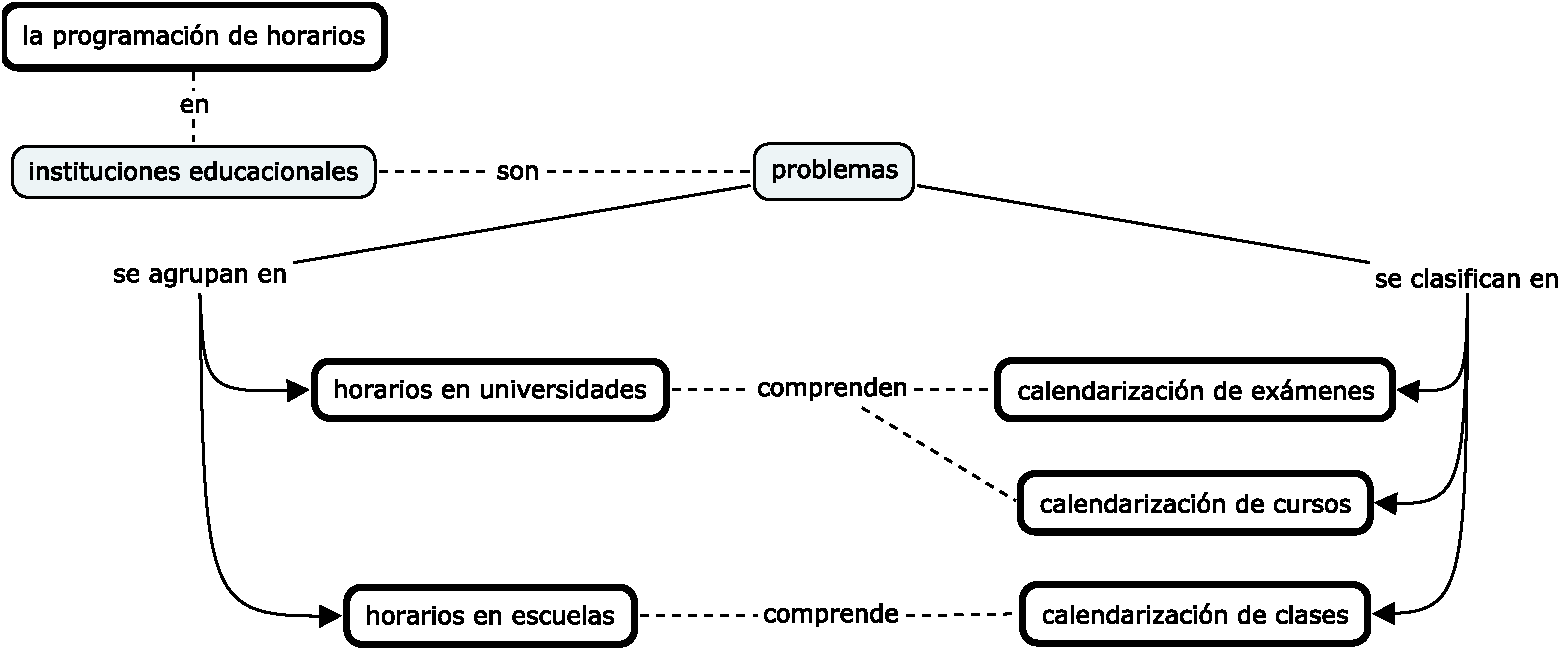
\includegraphics[width=\textwidth]{timetabling_classification.pdf}
\caption[Clasificación del problema]{Clasificación de los problemas en la elaboración de horarios educacionales}
\label{fig:timetabling_classification}
\end{figure}

\iffalse
Classification of Educational Timetabling Problems
Schaerf (1999a) classified educational timetabling into three main classes i.e. school timetabling, course timetabling and examination timetabling. They share the same basic characteristics of the general timetabling problem but can still have significant differences between them. Each one of them has its own constraints, requirements and rules. More details on educational timetabling can be found in Burke et al. (2004e). In this section, a classification of educational timetabling and its properties are discussed. We divided educational timetabling into two categories i.e. school timetabling and university timetabling (which consists of examination timetabling and course timetabling).
\fi

\subsubsection{Horarios en escuelas}

\index{horarios!en escuelas}

\paragraph{Horarios de clases}

\index{horarios!de clases}
De acuerdo a \citet[p.~88]{schaerf99a-survey-of-automated} el problema de horarios de clases consiste en calendarizar en un periodo semanal todas las clases de una escuela, evitando que los profesores se encuentren con dos clases al mismo tiempo, y viceversa. \citet[p.~10,11]{abdullah06heuristic-approaches} elabora explicando que el problema consiste de un conjunto de profesores, clases, lecciones y periodos semanales. En donde tales periodos semanales son predefinidos.

El problema intenta asignar lecciones a periodos y, un profesor a una clase en particular en un momento dado mientras se satisface un conjunto de restricciones con el fin producir un horario factible. Algunos ejemplos de restricciones en este tipo de problemas son las capacidades de alojamiento, ubicaciones, cargas de trabajo de los profesores, tiempo de descanso entre lecciones.

\subsubsection{Horarios en universidades}

\index{horarios!en universidades}\index{calendarización!de cursos}\index{calendarización!de exámenes}
El problema de la planificación de horarios en universidades puede ser agrupado en dos categorías: (i) calendarización de cursos y (ii) calendarización exámenes.
El problema de la calendarización de cursos es el proceso de la asignación de periodos y aulas de manera tal que las reuniones entre conferenciantes y estudiantes pueda ocurrir.
El problema de la calendarización de exámenes se refiere a la asignación de periodos y aulas de manera tal que los estudiantes puedan presentar sus exámenes.
Ambos problemas son similares de manera superficial, pero existen diferencias importantes que los distinguen.
En la calendarización de exámenes, múltiples exámenes pueden ser presentados en una misma aula (ej. auditorio) al mismo tiempo.
Sin embargo, esto no es posible para la calendarización de cursos en donde únicamente un curso puede ser asignado a un aula \citep[p.~11]{abdullah06heuristic-approaches}.

\paragraph{Calendarización de exámenes}

\index{calendarización!de exámenes}\index{calendarización!de cursos}
\citet[p.~4]{carter95recent-developments} definió el problema como la asignación de exámenes a un número limitado de periodos de manera tal que no existan conflictos o coincidencias. Los problemas de calendarización de cursos y exámenes son similares pero algunas diferencias relevantes según \citet[p.~159]{werra85an-introduction-to-timetabling} son:
\begin{enumerate}[a]
\item Existe generalmente un solo exámen por cada tema (mientras que hay varias exposiciones en un curso)
\item En la calendarización semanal de cursos, el objetivo principal es evitar conflictos (ej. la ocurrencia de que dos cursos elegidos por un mismo estudiante sean programados en el mismo periodo). Para los exámenes, generalmente se pide un máximo de un examen por día para cada estudiante o de ser posible, evitar la calendarización de exámenes en días consecutivos si el periodo de evaluación de exámenes lo permite.
\end{enumerate}
El problema de la calendarización de exámenes es muy común tanto en escuelas como en universidades. La asignación de los exámenes a los periodos está sujeta a un conjunto de limitaciones \citep[p.~12]{abdullah06heuristic-approaches}.

\paragraph{Calendarización de cursos}

\index{calendarización!de cursos}
El problema de la calendarización de cursos surge cuando una universidad (o incluso una escuela) ofrece una colección de cursos (cada uno consistiendo de un número dado de conferencias) sin existir un currículo fijo y en donde cada estudiante puede elegir cierto número de cursos. El problema consiste en la asignación de cada lectura a algún periodo en la semana de manera tal que ningún estudiante requiera asistir a más de una conferencia a la vez \citep[p.~157]{werra85an-introduction-to-timetabling}.
\citet[p.~88]{schaerf99a-survey-of-automated} define el problema como la calendarización semanal de todas las lecciones de un conjunto de cursos universitarios, minimizando los empalmes de las lecciones de cursos teniendo estudiantes en común.

\chapter{El gestor escolar}

section{Aplicaciones}

subsection{Métricas de desempeño}
subsection{Diagnóstico}
subsection{Multidisciplinario}

section{Factores de interés}

subsection{Laborales}

subsubsection{Regulatorios}


subsubsection{Interinstitucional}

subsection{Inversión}

subsubsection{Downsizing}

subsection{Económicos}

subsubsection{Utilidades}

subsubsection{Fiscales}

subsubsection{Aprovechamiento de recursos}

subsection{Sociales}

subsubsection{Involucramiento de paterfamilias}

subsection{Institucionales}

subsubsection{Profesorado}

subsection{Flexibilidad}

\chapter{Trabajo futuro y conclusiones}

\section{Resumen del trabajo de investigación}

\section{Contribuciones}

\section{Trabajo futuro}

\section{Diseminación}

\index{timetabling!university|see{programación de horarios en universidades}}
\index{timetabling!school|see{calendarización de clases y programación de horarios en escuelas}}
\index{timetabling!course|see{calendarización de cursos}}
\index{timetabling!examination|see{calendarización de exámenes}}

\index{scheduling|see{programación}}
\index{timetabling|see{calendarización}}

\index{schedule|see{programa}}
\index{sequence|see{secuencia}}
\index{timetable|see{horario}}

\appendix
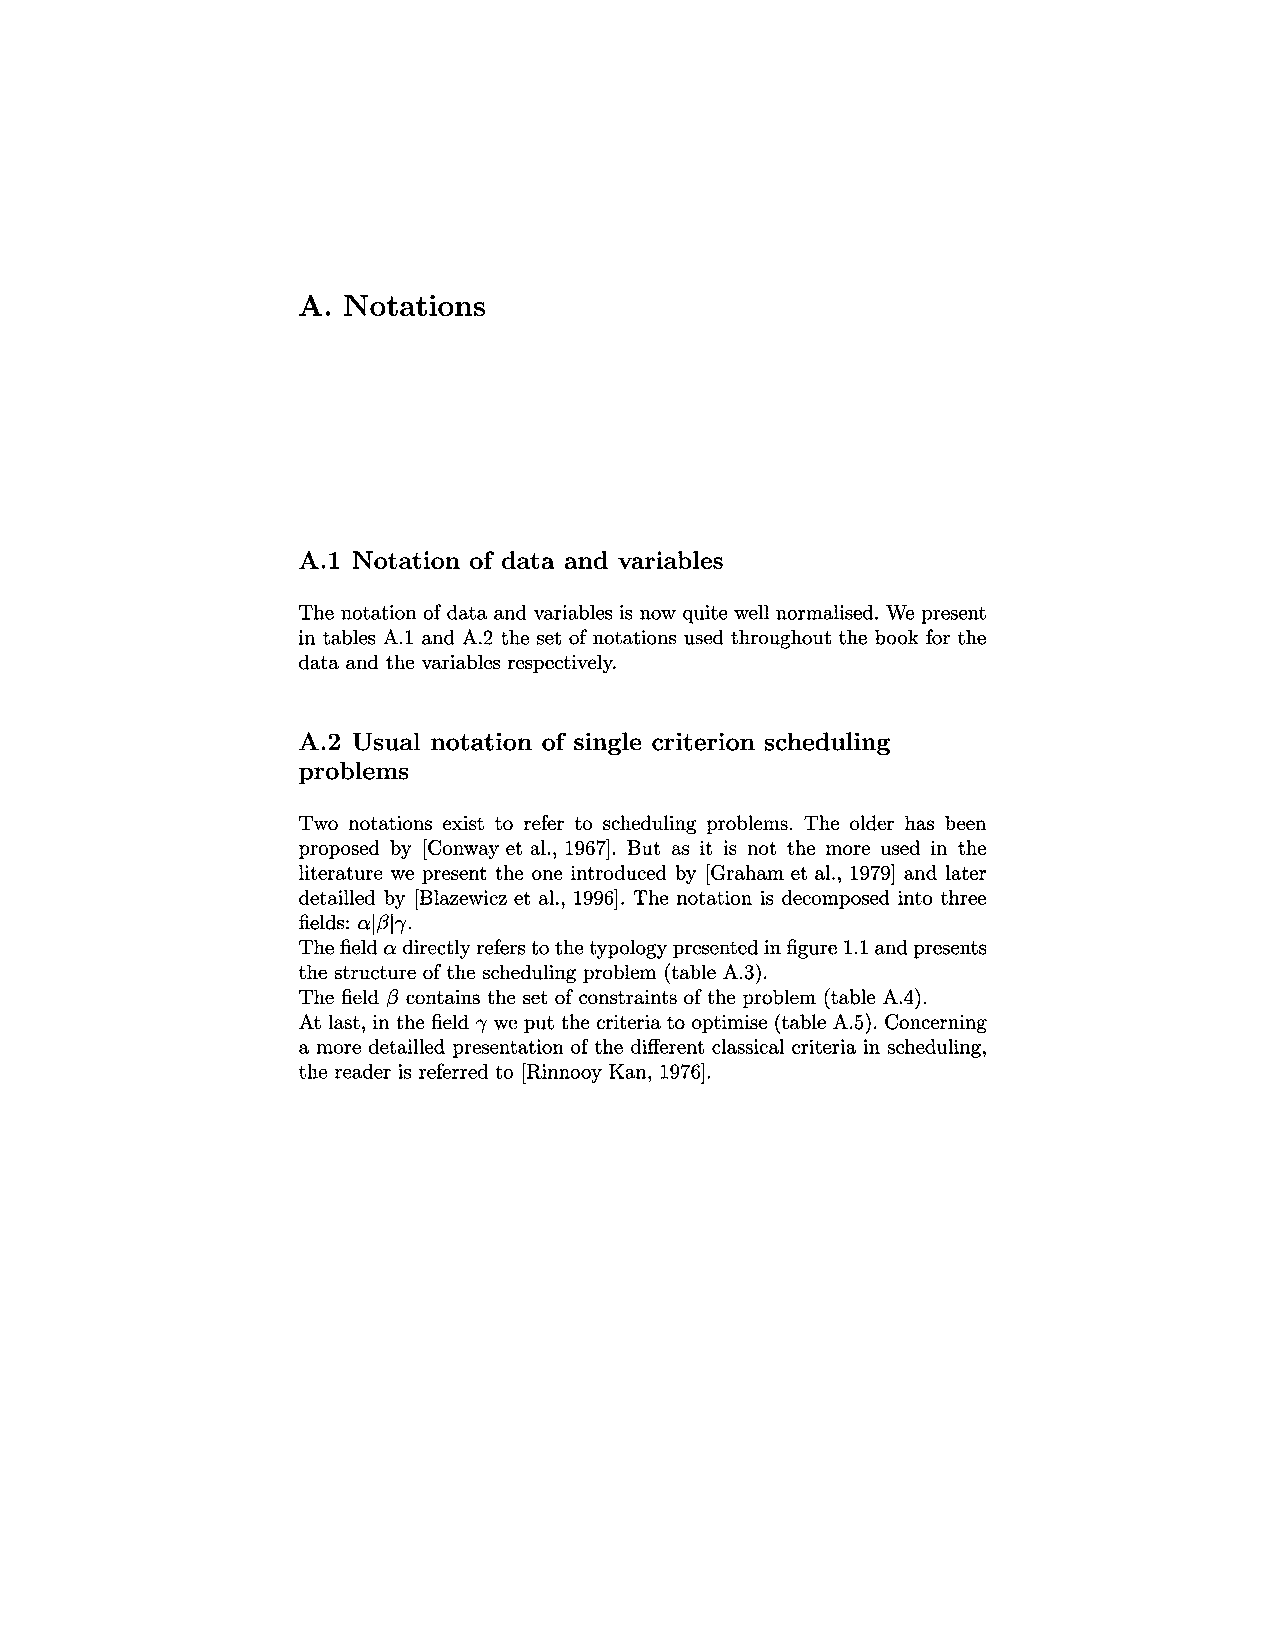
\includepdf[pages=-]{media/apendix_a.pdf}

% Bibliography
\bibliographystyle{apalike_modified}
\bibliography{bibliographies/reviewed,bibliographies/Dissertation_books}
{
\RaggedRight
\printindex
}
\end{document}
